\documentclass[compress,xcolor=table]{beamer}

\usepackage{lmodern}
\usepackage[utf8]{inputenc}

\mode<presentation>
{
	\usetheme{Madrid}      % or try Darmstadt, Madrid, Warsaw, ...
	\usecolortheme{seahorse} % or try albatross, beaver, crane, ...
	\usefonttheme{serif}  % or try serif, structurebold, ...
	\setbeamertemplate{navigation symbols}{}
	\setbeamertemplate{caption}[numbered]
} 

\makeatletter
\setbeamertemplate{headline}{%
	\begin{beamercolorbox}[ht=2.25ex,dp=3.75ex]{section in head/foot}
		\insertnavigation{\paperwidth}
	\end{beamercolorbox}%
}%
\makeatother

\makeatletter
\newenvironment{withoutheadline}{
	\setbeamertemplate{headline}[default]
	\def\beamer@entrycode{\vspace*{-\headheight}}
}{}
\makeatother

\usepackage[english]{babel}
\usepackage[utf8]{inputenc}
\usepackage{xcolor}
\usepackage{listings}
\usepackage{textpos}
\newcommand\citem[1]{\item[{[#1]}] }

\lstset
{
	language=[LaTeX]TeX,
	breaklines=true,
	basicstyle=\tt\scriptsize,
	%commentstyle=\color{green}
	keywordstyle=\color{red},
	%stringstyle=\color{black}
	identifierstyle=\color{orange},
}

\newcommand{\backupbegin}{
	\newcounter{finalframe}
	\setcounter{finalframe}{\value{framenumber}}
}
\newcommand{\backupend}{
	\setcounter{framenumber}{\value{finalframe}}
}

\newenvironment<>{varblock}[2][.9\textwidth]{%
	\setlength{\textwidth}{#1}
	\begin{actionenv}#3%
		\def\insertblocktitle{#2}%
		\par%
		\usebeamertemplate{block begin}}
	{\par%
		\usebeamertemplate{block end}%
\end{actionenv}}

%\usepackage{outlines}
\setbeamercolor{itemize item}{fg=red,bg=white}

\usepackage{multirow}
\usepackage{caption}
\usepackage{subcaption}

\usepackage{animate}

\newcommand\pro{\item[$+$]}
\newcommand\con{\item[$-$]}

\usepackage[edges]{forest}
\usetikzlibrary{shadows,arrows.meta}
\usepackage{tcolorbox}
%Defining the styles used in trees
%Note that the fill colour is not defined here.
\tikzset{parent/.style={align=center,text width=2cm,rounded corners=2pt},
	child/.style={align=center,text width=7.5cm,rounded corners=6pt},
	grandchild/.style={align=left, text width=13cm}
}

\newcommand\blfootnote[1]{%
	\begingroup
	\renewcommand\thefootnote{}\footnote{#1}%
	\addtocounter{footnote}{-1}%
	\endgroup
}

%%% TITLE
\title[PIMRC 2021]{Discrete-Time Analysis of\\Wireless Blockchain Networks}
\author[Wilhelmi, F., and Giupponi, L.]{
\includegraphics[width=\textwidth,height=0.13\textheight,keepaspectratio]{img/cttc}\\~\\ \textbf{Francesc Wilhelmi} and Lorenza Giupponi}
\institute[]{2021 IEEE International Symposium on Personal, Indoor and Mobile Radio Communications (IEEE PIMRC 2021)}
\date[13-16 September 2021]{13-16 September 2021}

\AtBeginSection[]
{
	\begin{frame}<beamer>
	\frametitle{Outline}
	\tableofcontents[currentsection,currentsubsection]
\end{frame}
}

\begin{document}

\begin{withoutheadline}
	\begin{frame}
		\titlepage
	\end{frame}
\end{withoutheadline}

\begin{frame}{Table of contents} % and our simple frame
	\tableofcontents
\end{frame}

%%%%%%%%%%%%%%
%%% Motivation
%%%%%%%%%%%%%%
\section[Introduction]{Introduction and Related Work}

\subsection{}
\begin{frame}{Towards Blockchain-enabled Communications}
	\begin{block}{Network sharing in 5G/6G}
			\begin{itemize}
				\item Economic sustainability
				\item Need for automation to exchange network resources
				\item Need for trust
			\end{itemize}
		\end{block}	
		\begin{exampleblock}{Blockchain}
			\begin{itemize}
				\item Immutability, transparency, and security
				\item Exchange resources in 5G/6G
				\item Important challenges (computation, energy, delay, scalability)
			\end{itemize}
		\end{exampleblock}	
		\begin{center}
	\begin{minipage}{10cm}
		\begin{alertblock}{}
			\centering
			\scriptsize \textbf{Need for understanding the impact of BC over wireless networks}
		\end{alertblock}
	\end{minipage}
\end{center}
\end{frame}

\subsection{}
\begin{frame}{Main contributions}

\begin{columns}
		\begin{column}{5cm}
		\begin{figure}
			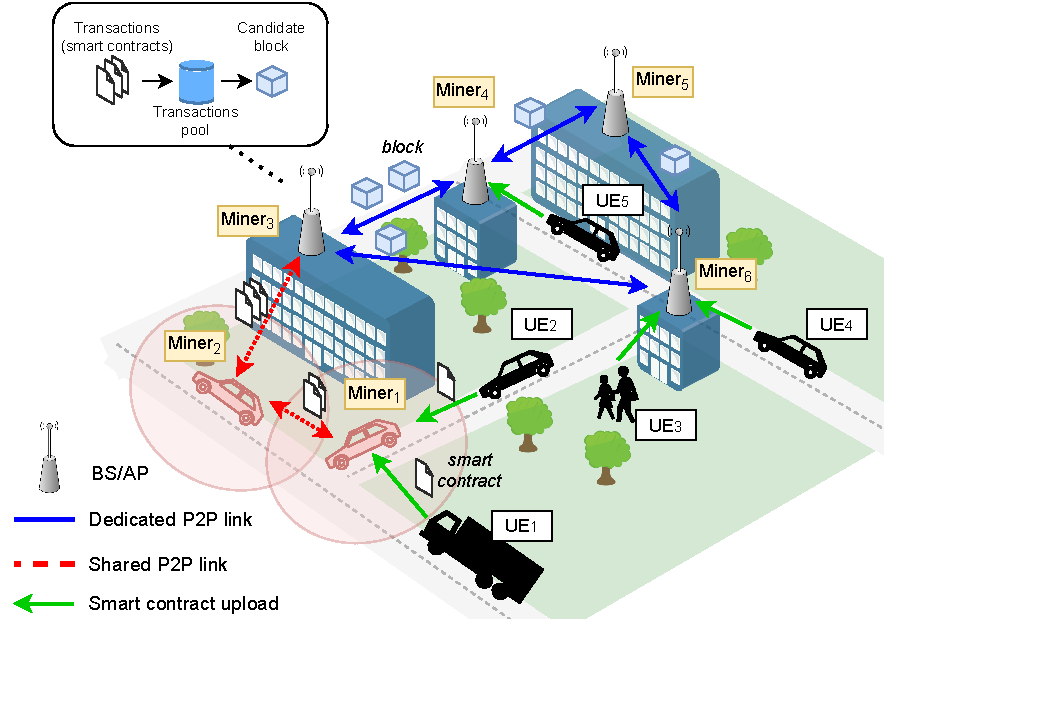
\includegraphics[width=\textwidth,keepaspectratio]{img/blockchain_ecosystem}\caption{\scriptsize Envisioned BC-enabled RAN ecosystem}
		\end{figure}
	\end{column}
	\begin{column}{6.7cm}
		\begin{enumerate}
			%\pause
			\item Open, flexible BC RAN ecosystem%End users are not necessarily bound to a specific operator in the long term but, at any moment, can trigger requests to get specific data services. Based on the BC technology, the User Equipment (UE) devices issue smart contracts that facilitate automatic, transparent, and auditable mechanisms whereby operators and service providers fulfill UE requests. The smart contracts (including service indicators such as duration, maximum latency, or throughput) are registered in a public BC, which enables flexible and decentralized on- demand network access.
			%\pause
			\item Batch-service queue model for BC
			%\pause
			\item Model validation
			%\pause
			\item Insights on Wireless BC Networks
		\end{enumerate}
	\end{column}
\end{columns}
	\vspace{-0.5cm}
	%\pause
	\begin{minipage}{12cm}
	\begin{alertblock}{}
		\scriptsize All the source code used in this project is of open access and completely available:
		\begin{itemize}
			\item BC batch-service queue simulator: \url{https://github.com/fwilhelmi/batch_service_queue_simulator}
			\item Model implementation: \url{https://bitbucket.org/francesc_wilhelmi/model_blockchain_delay}		
	\end{itemize}
	\end{alertblock}
\end{minipage}
\end{frame}

\subsection{}
\begin{frame}{Important references}
	\begin{exampleblock}{Blockchain characterization}
		\begin{itemize}
			\item Simulation, analytical model, traces
			\item Broad survey: \cite{fan2020performance}
		\end{itemize}		
	\end{exampleblock}
	\begin{block}{Markov processes and batch service queuing}			
		\begin{itemize}
			\item Packets leave the queue in batches, rather than individually
			\item Baseline works: \cite{kawase2017transaction,kawase2018batch,li2018blockchain,geissler2019discrete,li2019markov}
		\end{itemize}			
	\end{block}
\begin{alertblock}{Our contribution}			
	\begin{itemize}
		\item We model queue states at departure instants% provide a more detailed performance evaluation of BC
		\item We incorporate the key effects of timers and forks % To the best of our knowledge, none of these features has been considered before in any BC model. We believe that these features are fundamental to any BC model for multiple reasons. First, timers are important to break the dependence of the mining procedure on the arrivals rate, which allows guaranteeing a maximum waiting delay, even if blocks are not filled with transactions (i.e., blocks are mined periodically). Disregarding the effects of timers leads to poor accuracy when deriving the queue status (e.g., the number of transactions in it) or the expected delay [26]. Second, the forks are a dramatic source of instability in BC. The appropriate modeling of their behavior ensures high accuracy and fidelity to capture the BC network’s real dynamics.
	\end{itemize}			
\end{alertblock}

\end{frame}


%%%%%%%%%%%%%%
%%% SYSTEM MODEL
%%%%%%%%%%%%%%
\section{System Model}

%In the proposed BC-enabled communication environment, peers (miners) generate candidate blocks with transactions (service requests) from the UEs, which are mined once the block size SB is reached, or when a timer Tw expires. To mine a block, peer nodes run a given consensus mechanism such as Proof-of-Work (PoW) and then propagate it over the P2P network. Upon successful block propagation, the winning miner is allowed to append the candidate block to the BC.
\subsection{}
\begin{frame}{Blockchain-enabled RAN delays}
\begin{columns}
	\begin{column}{6cm}
		Transaction \textbf{confirmation} latency:
		\begin{enumerate}
			\item Smart contract upload ($T_\text{up}$)
			\item Queuing ($T_\text{q}$)
			\item Block generation ($T_\text{bg}$)
			\item Block propagation ($T_\text{bp}$)
		\end{enumerate}
	\end{column}
	%\pause
	\begin{column}{5cm}
		\begin{figure}
			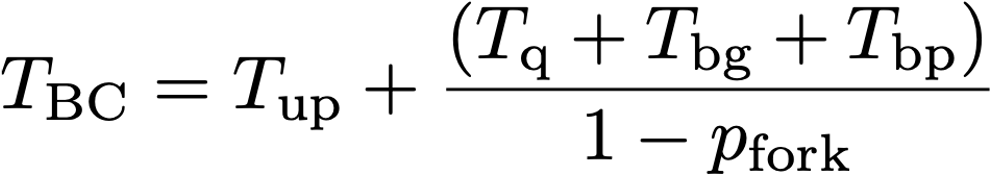
\includegraphics[width=\textwidth,keepaspectratio]{img/equation_delay}
		\end{figure}
	\end{column}
\end{columns}
\end{frame}

%%%%%%%%%%%%%%
%%% SYSTEM MODEL
%%%%%%%%%%%%%%
\section{Batch Service Queue Model}

\subsection{}
\begin{frame}{Queue behavior}
	\begin{block}{Overview}
		\begin{itemize}
			\item Finite-length $M/M^s/1/K$ queue
			\item Departures conditioned to arrivals ($\lambda$), block size ($S^B$), mining timeout ($T_w$), and mining rate ($\mu$)
			\item Goal: find expected queue occupancy
		\end{itemize}
	\end{block}		
	\begin{figure}
		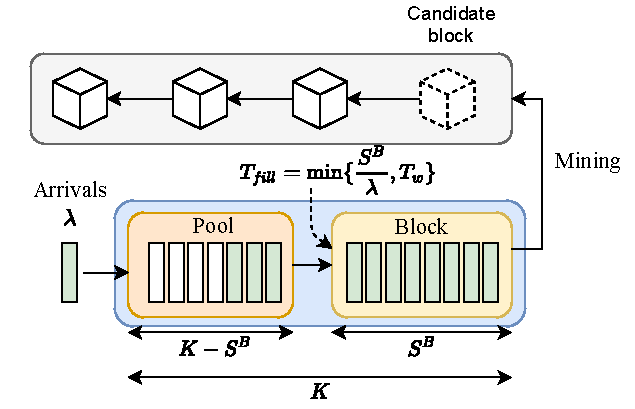
\includegraphics[width=0.45\textwidth,keepaspectratio]{img/batch_service_queue}\caption{\scriptsize Blockchain queue}
	\end{figure}
\end{frame}

\subsection{}
\begin{frame}{Markov model}
\begin{columns}
	\begin{column}{5.5cm}
		\begin{block}{Steps}
			\begin{enumerate}
				\item Find departures distribution ($\boldsymbol{\pi}^d$)
				\item Get steady-state distribution ($\boldsymbol{\pi}^s$)
				\item Compute expected queue occupancy and delay
			\end{enumerate}
		\end{block}
	\end{column}
	\begin{column}{5.5cm}
		\begin{exampleblock}{Forks}
			\begin{enumerate}
				\item Concurrent miners affect to the mining rate ($\text{E}[X_{(1)}] = \frac{1}{n\mu}$)
				\item Transactions involved in forks are re-added to the queue %impact on the transition prob. matrix
			\end{enumerate}
		\end{exampleblock}		
	\end{column}
\end{columns}
\begin{figure}
	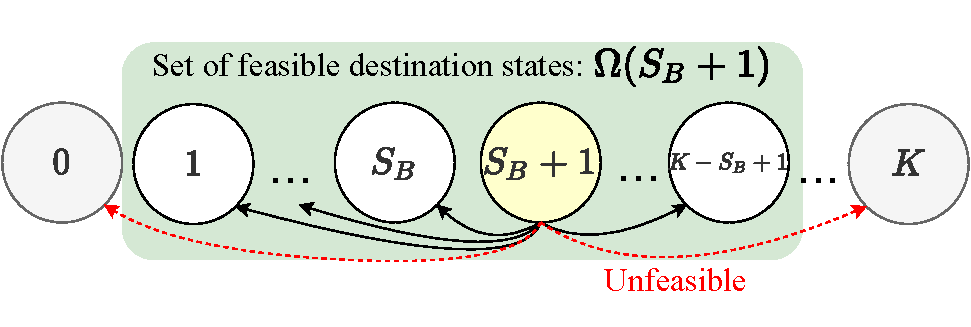
\includegraphics[width=0.55\textwidth,keepaspectratio]{img/markov_chain_1}\caption{\scriptsize Inter-departure states}
\end{figure}
\end{frame}

%%%%%%%%%%%%%%
%%% PERF. EVALUATION
%%%%%%%%%%%%%%
\section{Performance Evaluation}

\subsection{}
\begin{frame}{Simulation scenario}
\begin{columns}
	\begin{column}{6.5cm}
		\begin{block}{Scenario}
			\begin{itemize}
				\item Random cellular  deployment
					\begin{itemize}
						\item 19 BS acting as miners
					\end{itemize}
				\item BC links
				\begin{itemize}
					\item IEEE 802.11ax (UE-BS)
					\item 5G NR X2/Xn (P2P)
				\end{itemize}
				\item Characterize the delay for different BC parameters
			\end{itemize}
		\end{block}
	\end{column}
	\begin{column}{4.5cm}
		\begin{figure}
			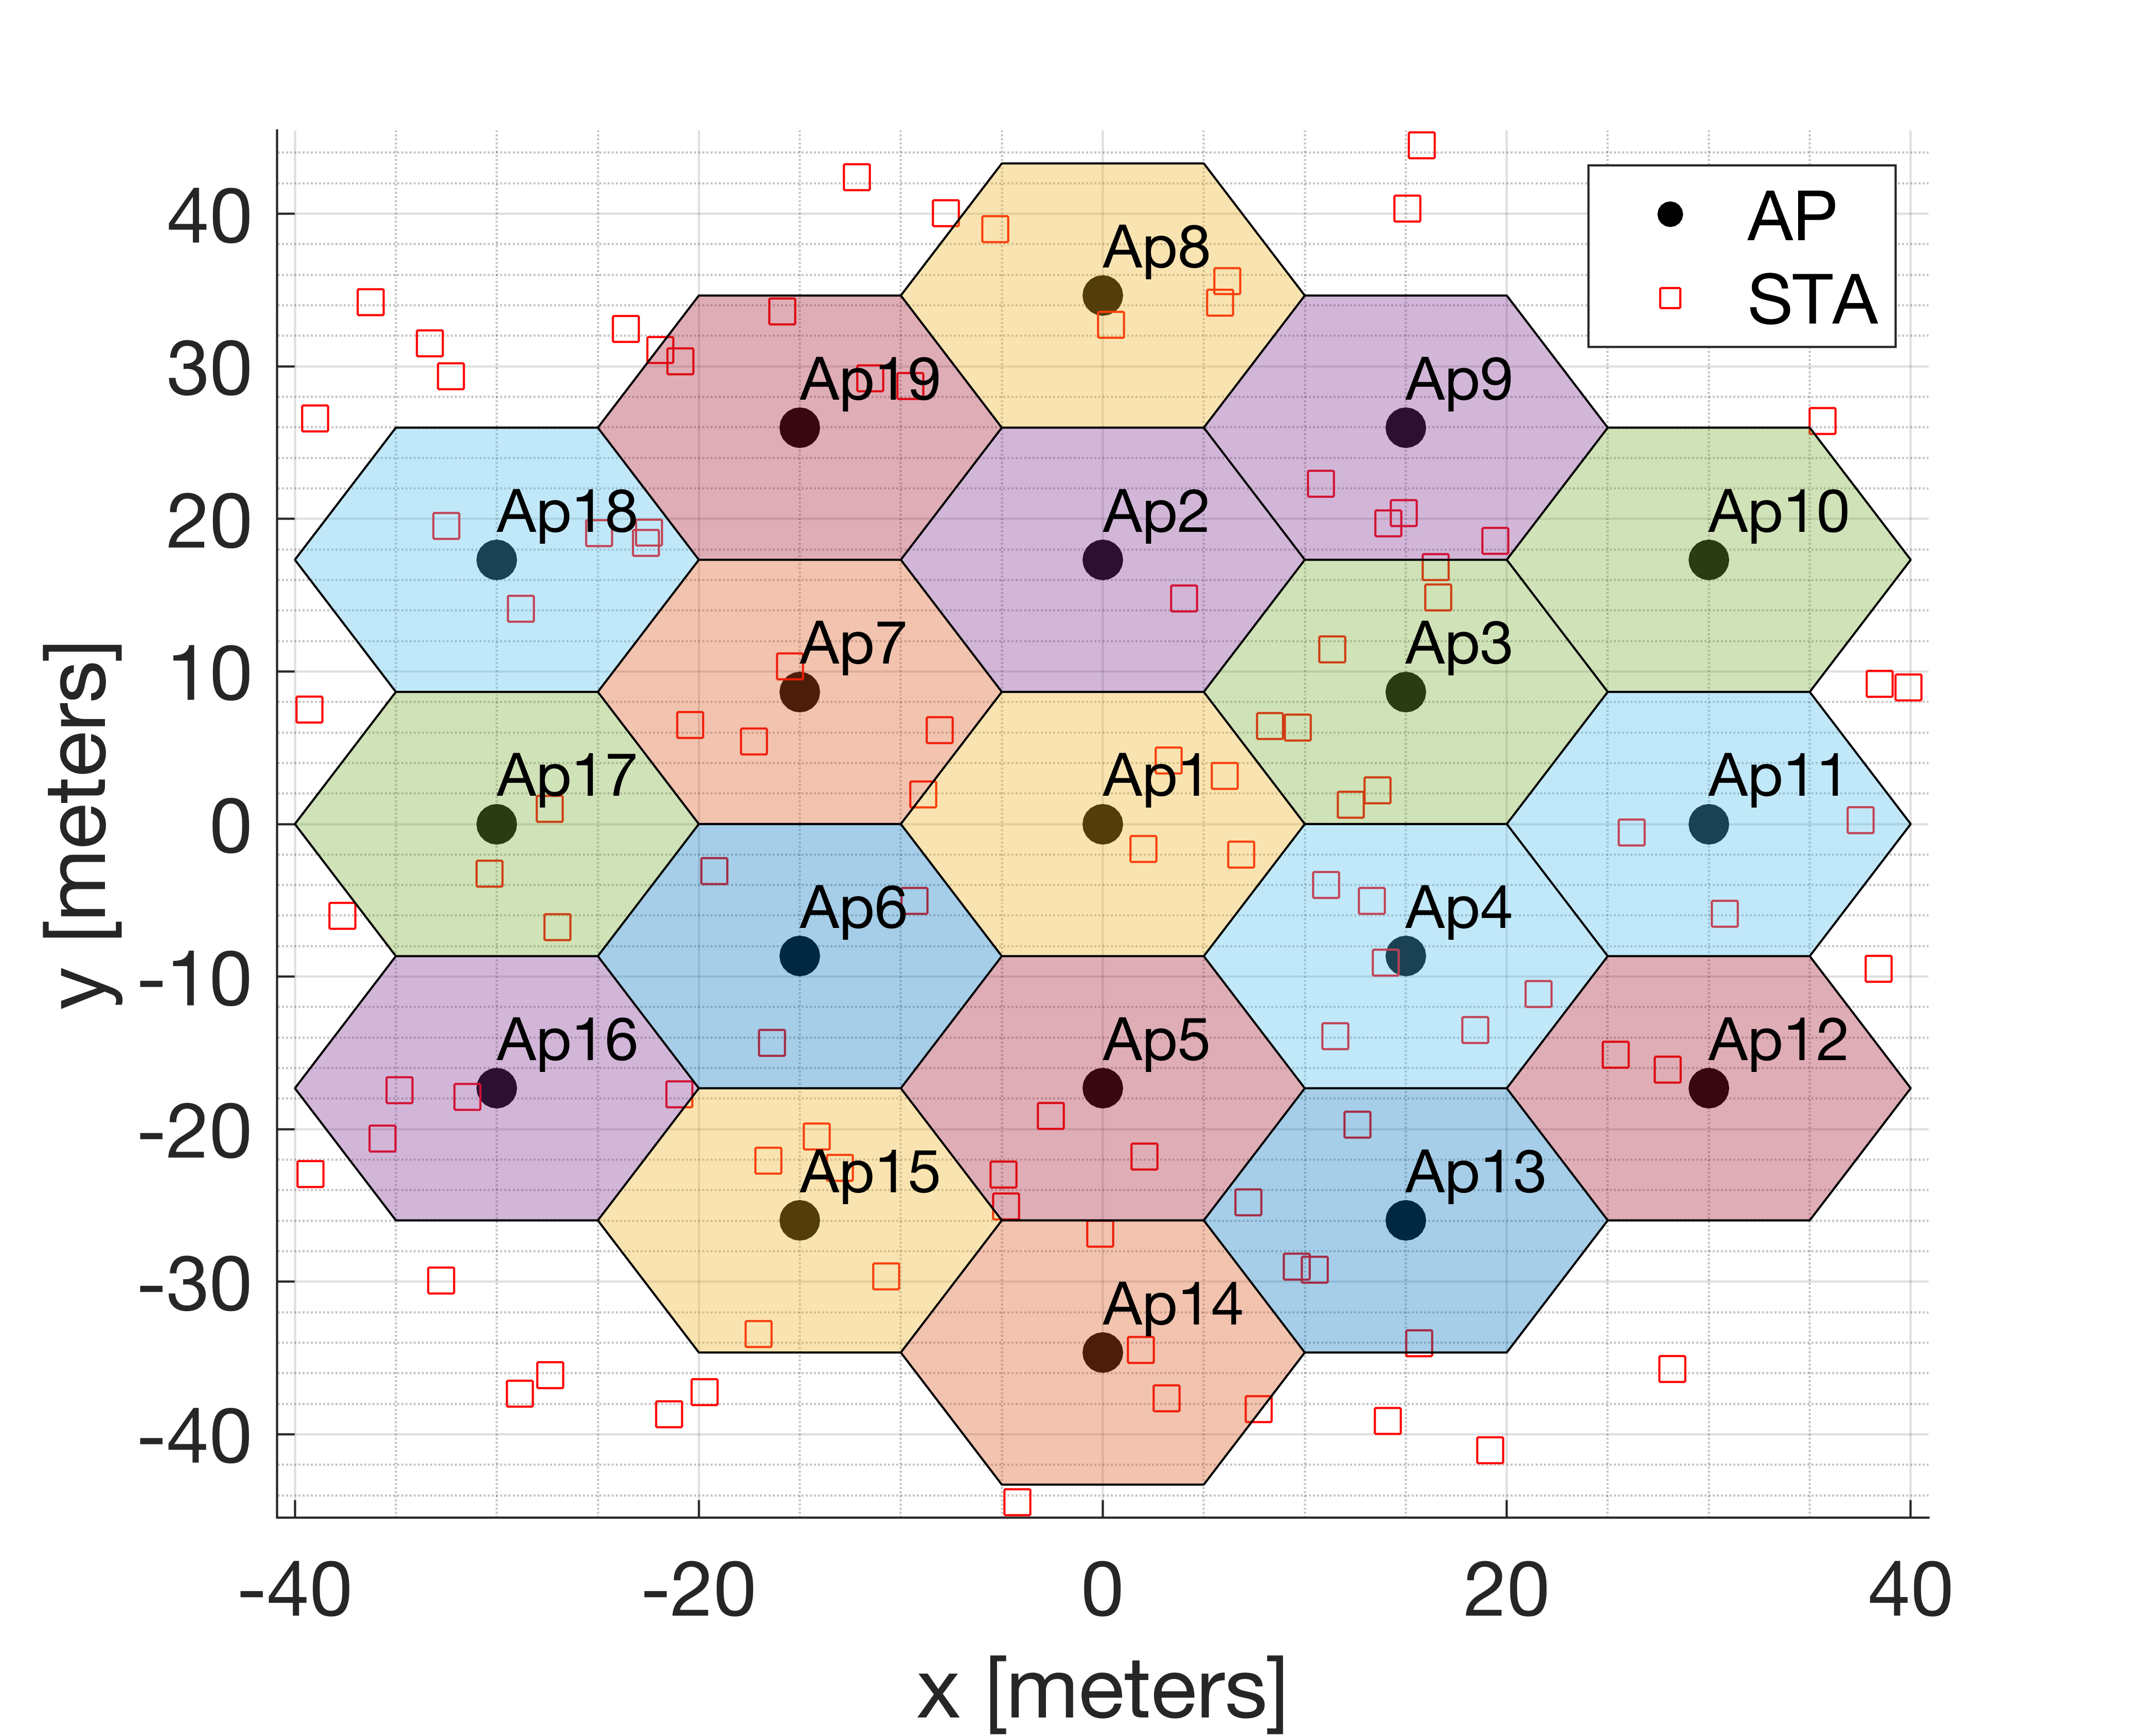
\includegraphics[width=\textwidth,keepaspectratio]{img/random_deployment}\caption{\scriptsize Simulation scenario}
		\end{figure}
	\end{column}
\end{columns}
\end{frame}

\subsection{}
\begin{frame}{Validation of the queuing delay}
\begin{columns}
	\begin{column}{5.5cm}
		\begin{figure}
			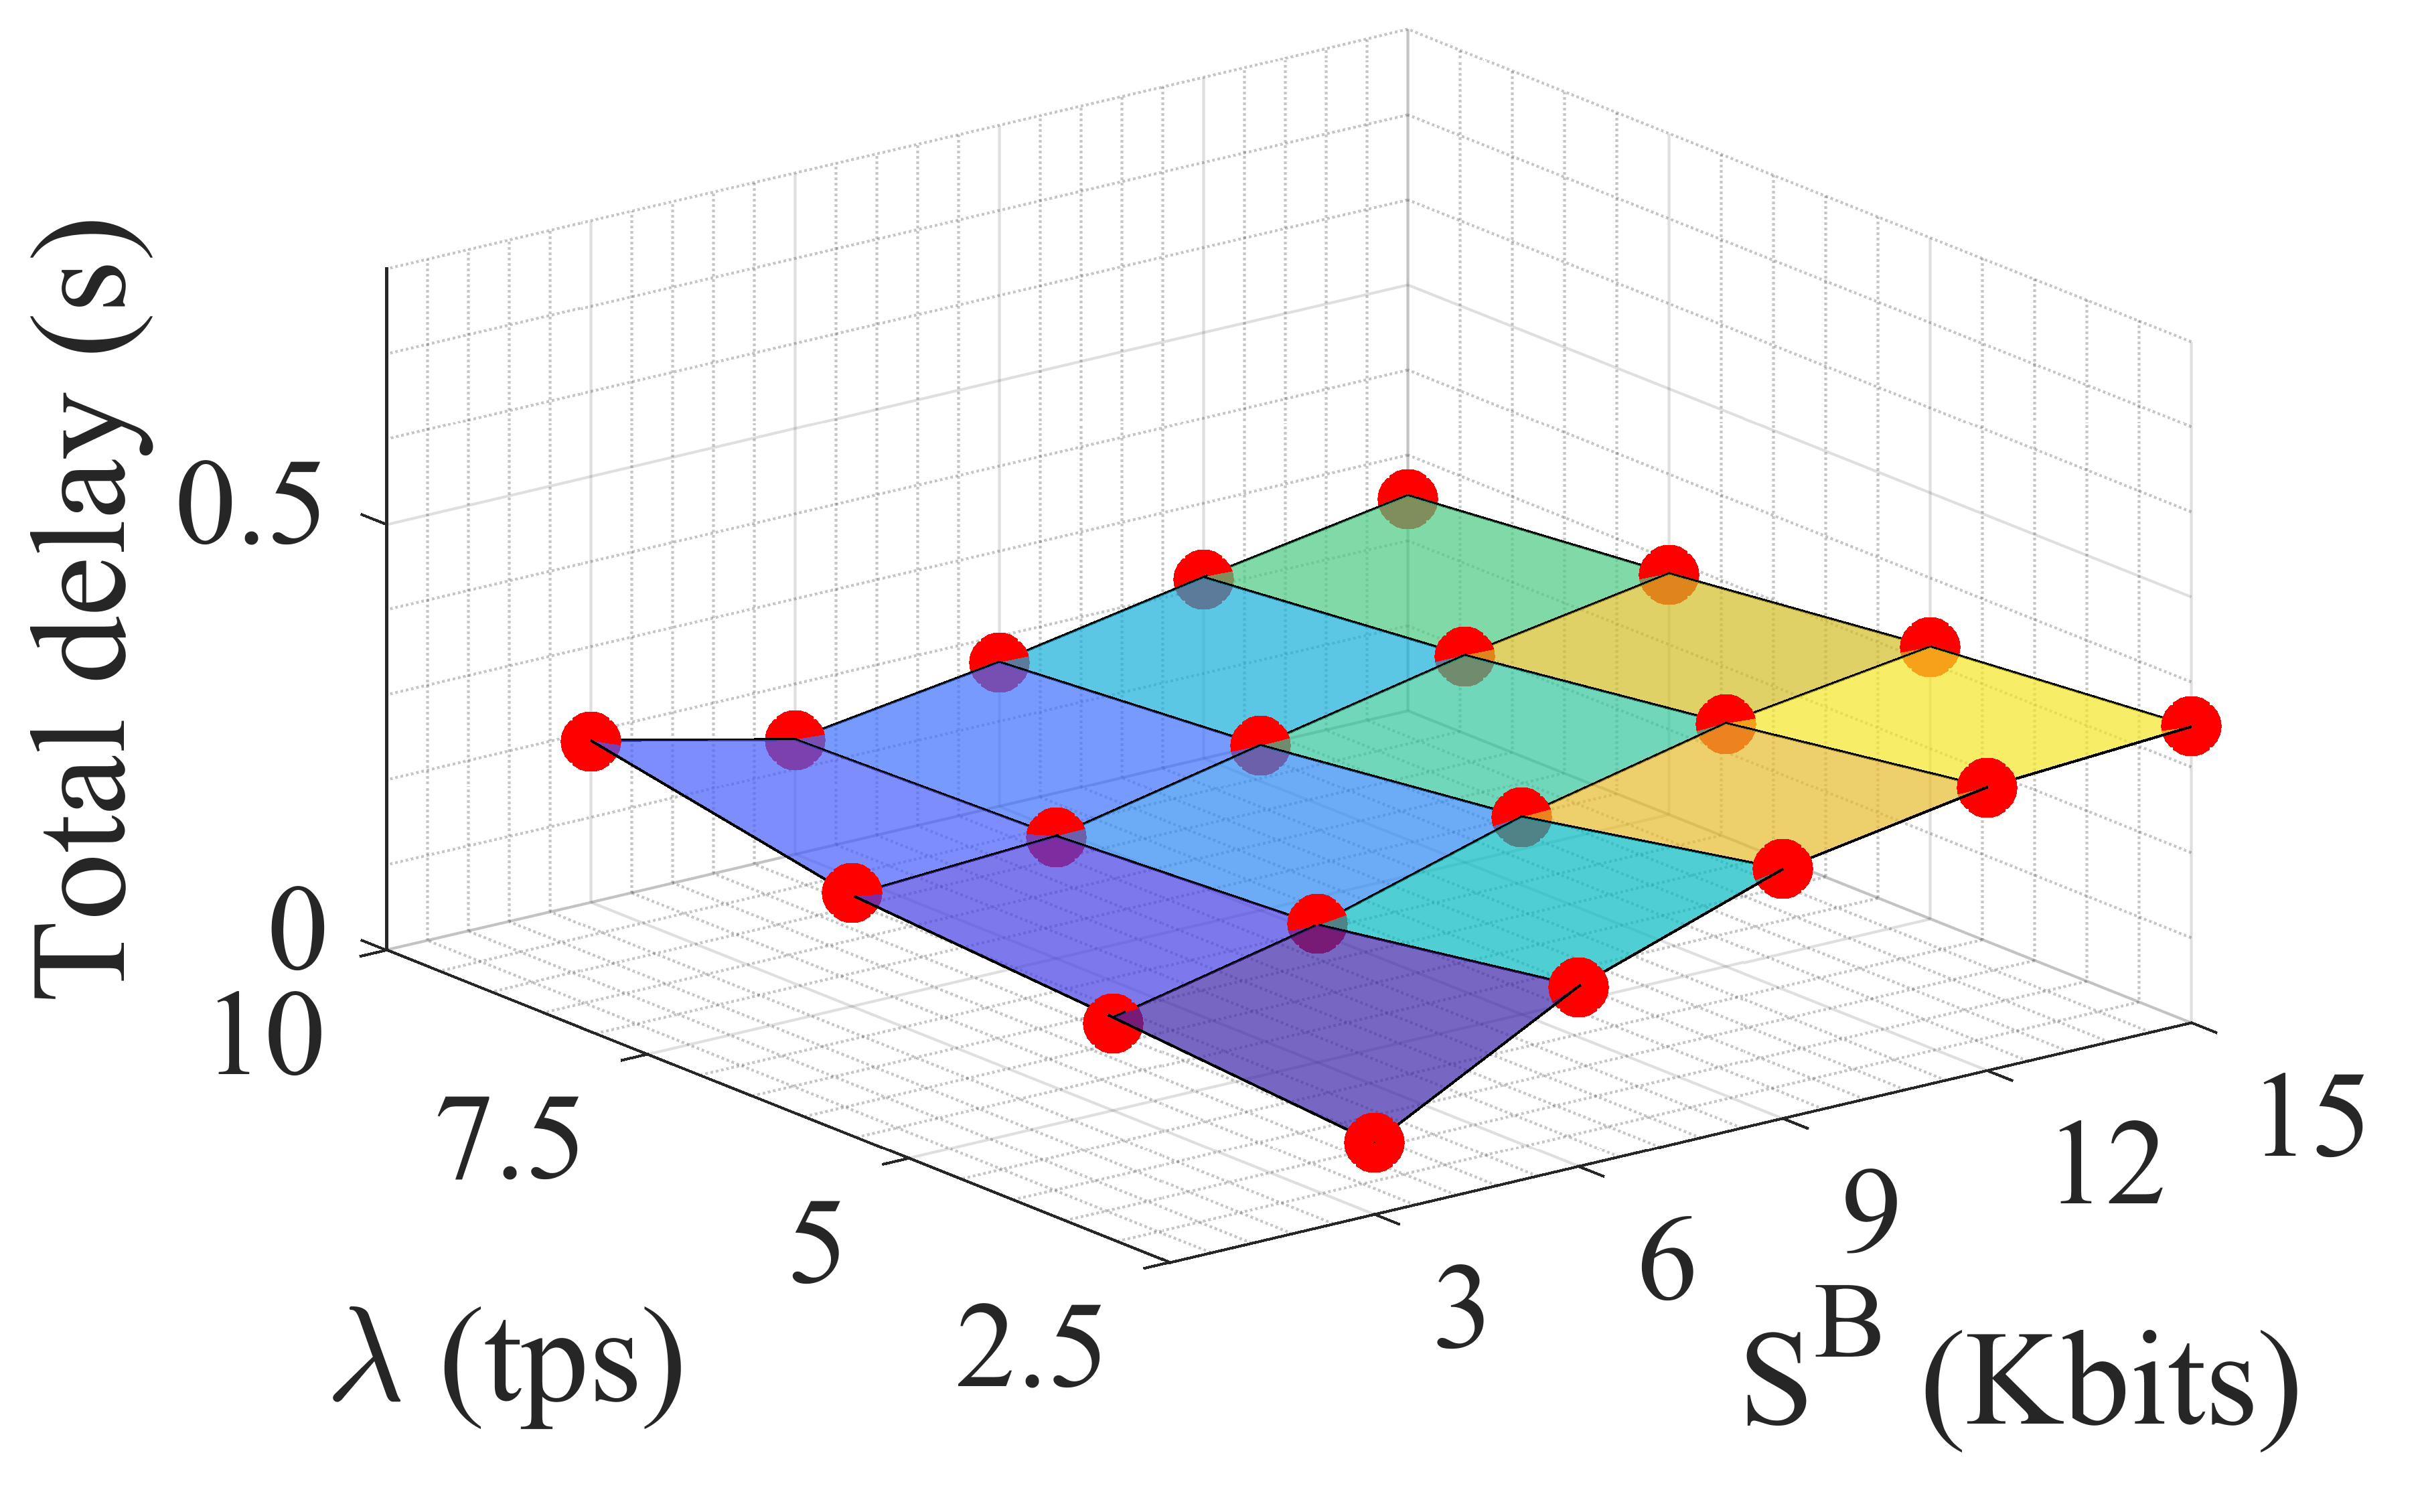
\includegraphics[width=0.7\textwidth,keepaspectratio]{img/total_delay_forks0_tw01}\caption{\scriptsize $T_w=0.5$ s, forks disabled}
		\end{figure}
	\end{column}
	\begin{column}{5.5cm}
		\begin{figure}
			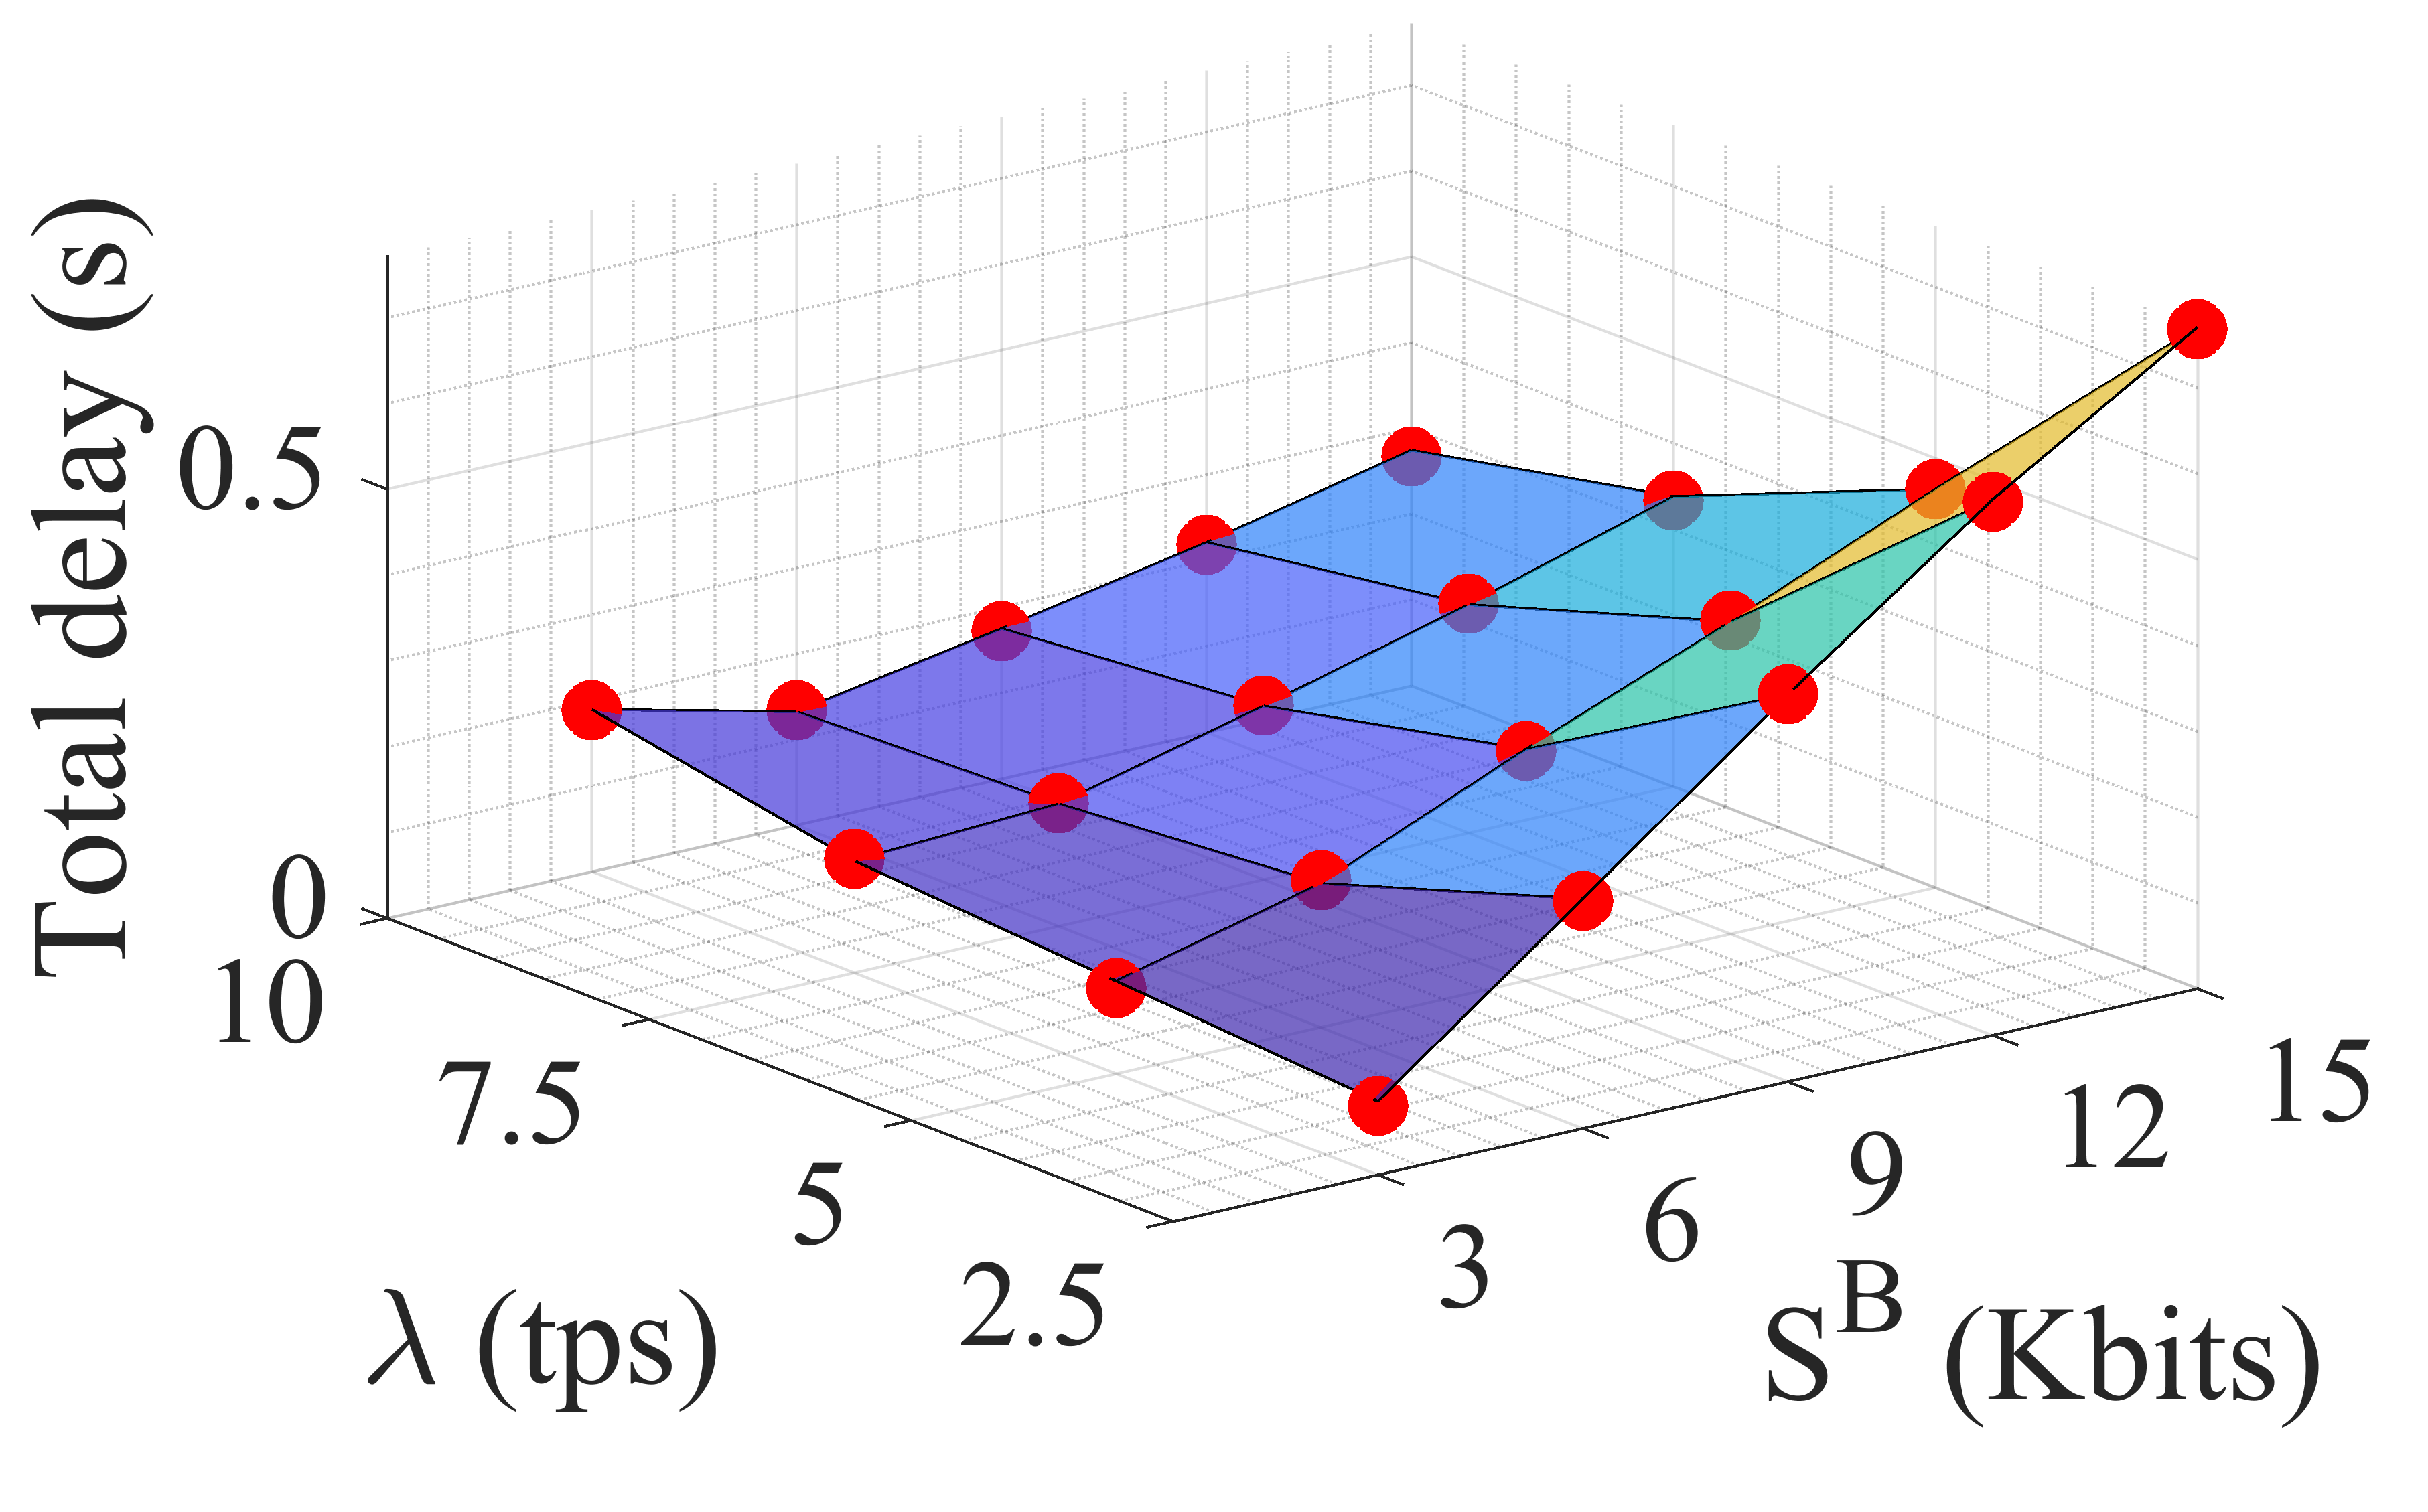
\includegraphics[width=0.7\textwidth,keepaspectratio]{img/total_delay_forks0_tw2}\caption{\scriptsize $T_w=2$ s, forks disabled}
		\end{figure}
	\end{column}
\end{columns}
\begin{columns}
	\begin{column}{5.5cm}
		\begin{figure}
			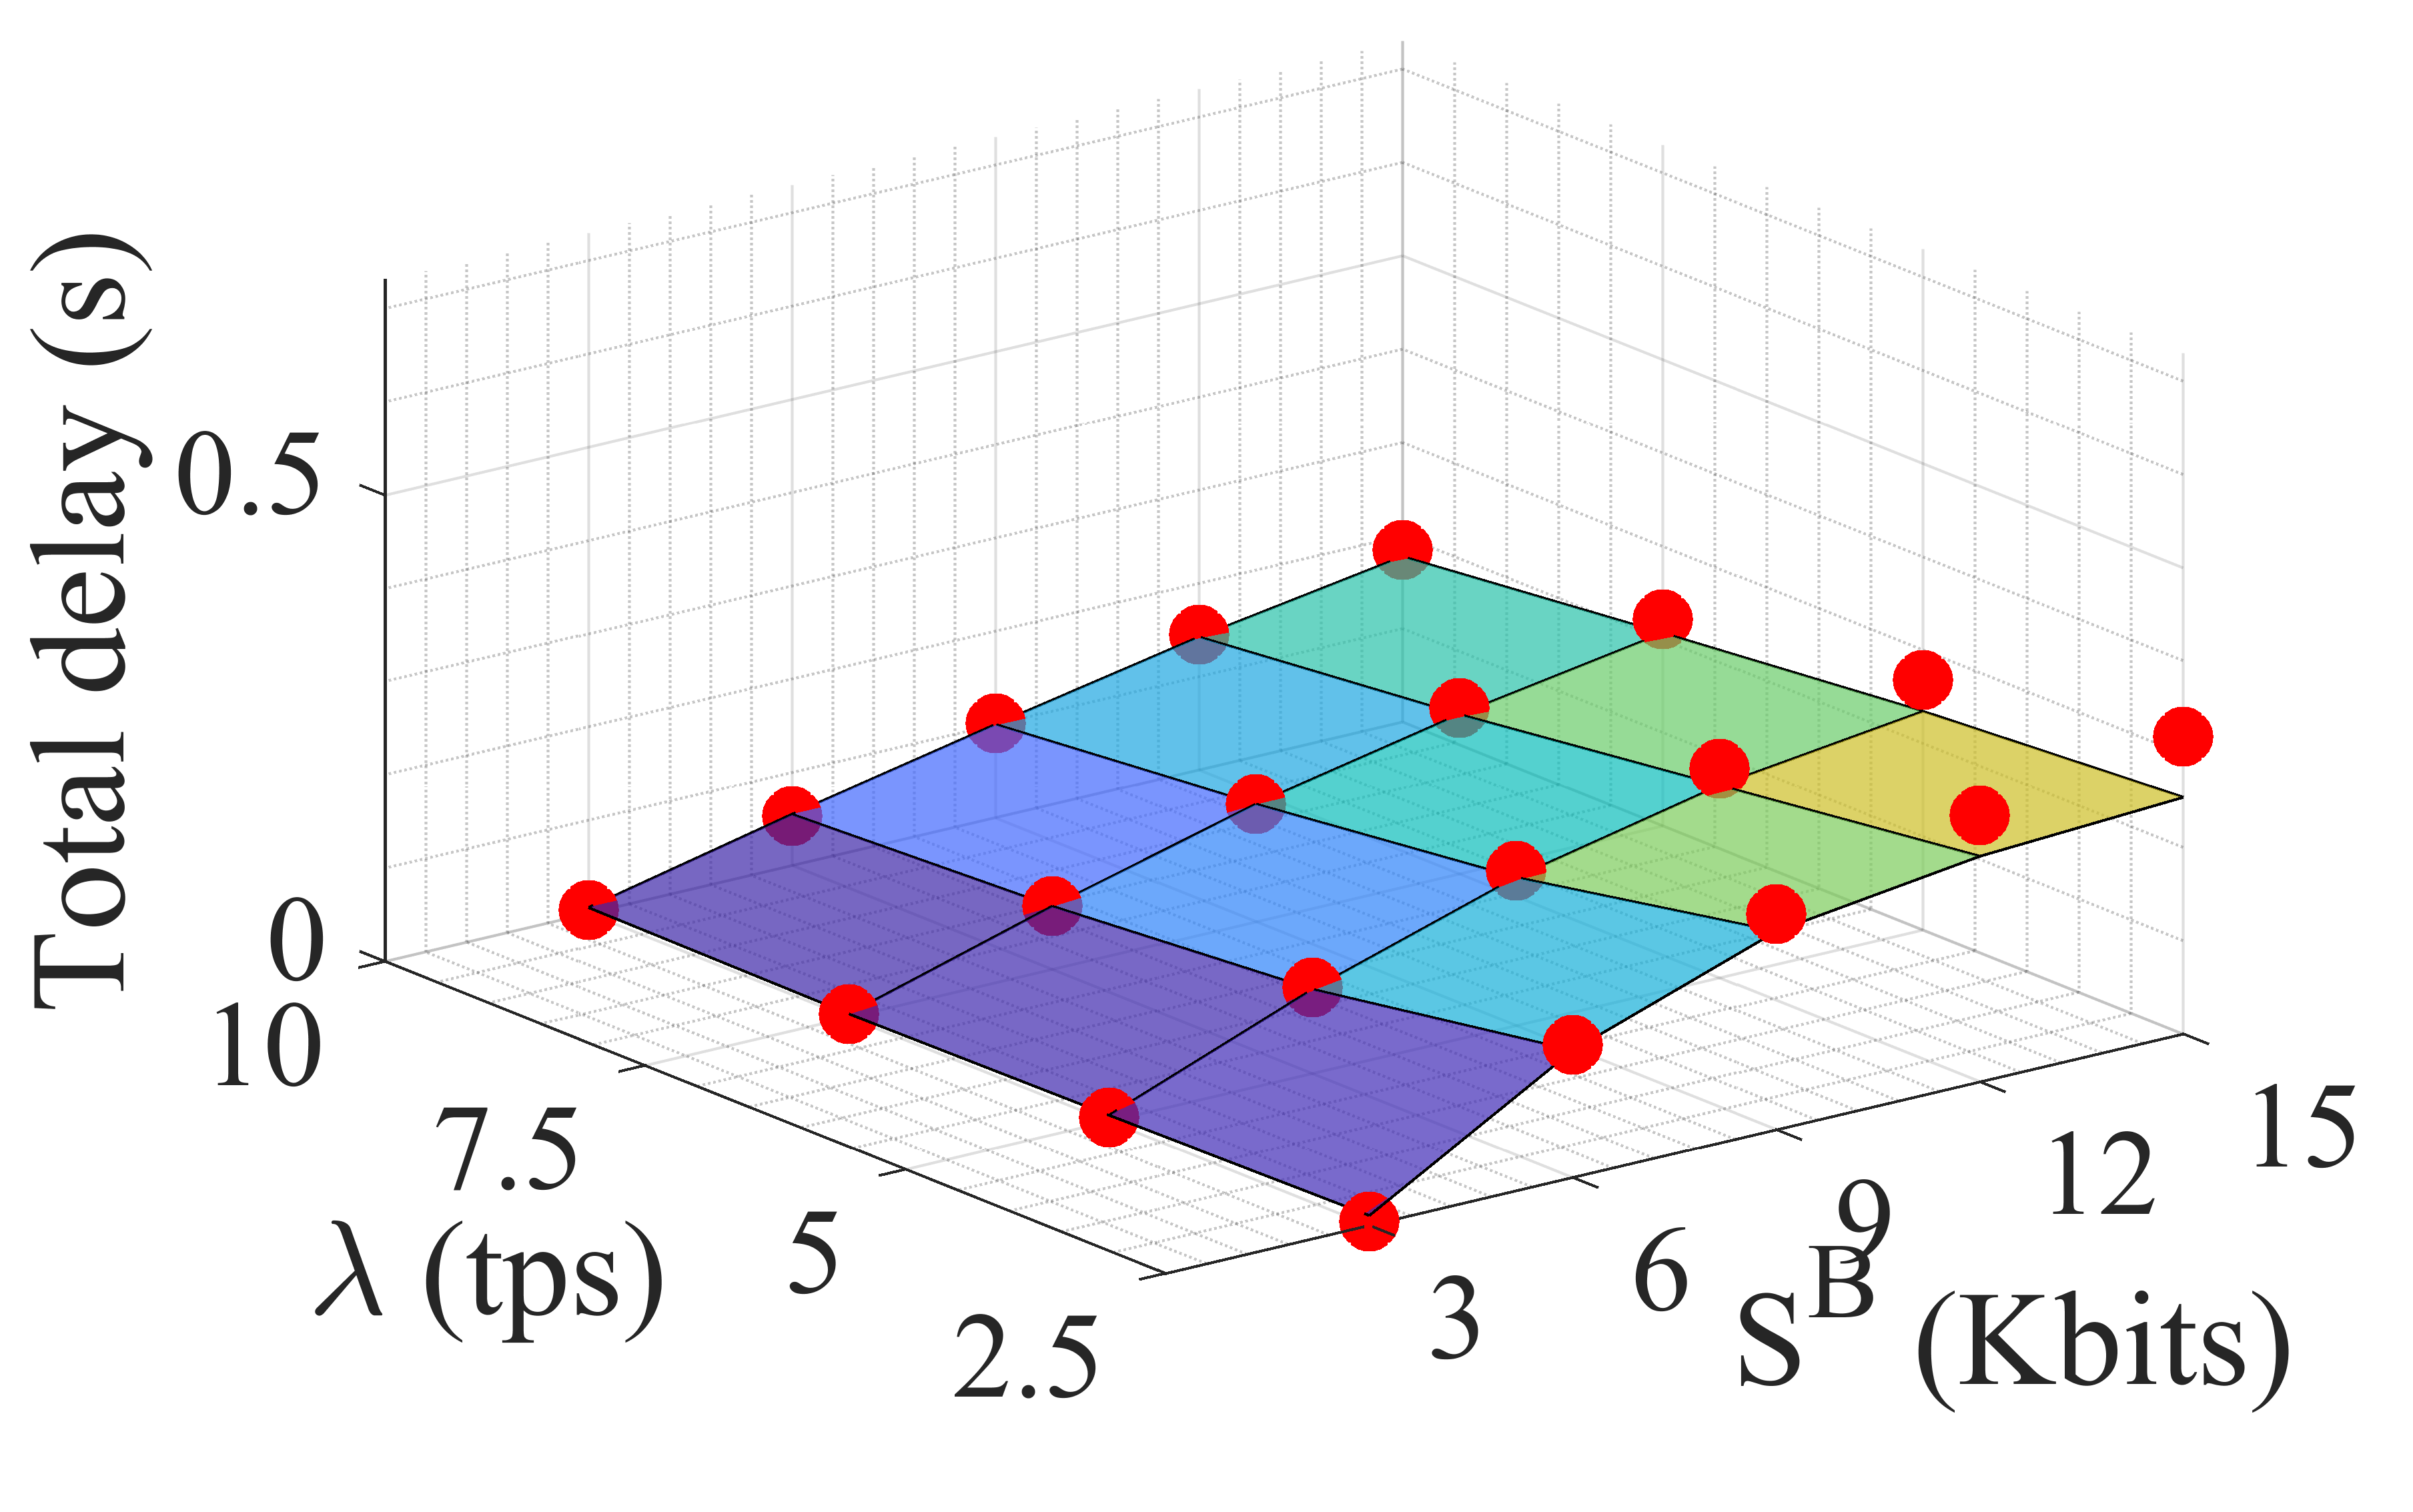
\includegraphics[width=0.7\textwidth,keepaspectratio]{img/total_delay_forks1_tw05}\caption{\scriptsize $T_w=0.5$ s, forks enabled}
		\end{figure}
	\end{column}
	\begin{column}{5.5cm}
		\begin{figure}
			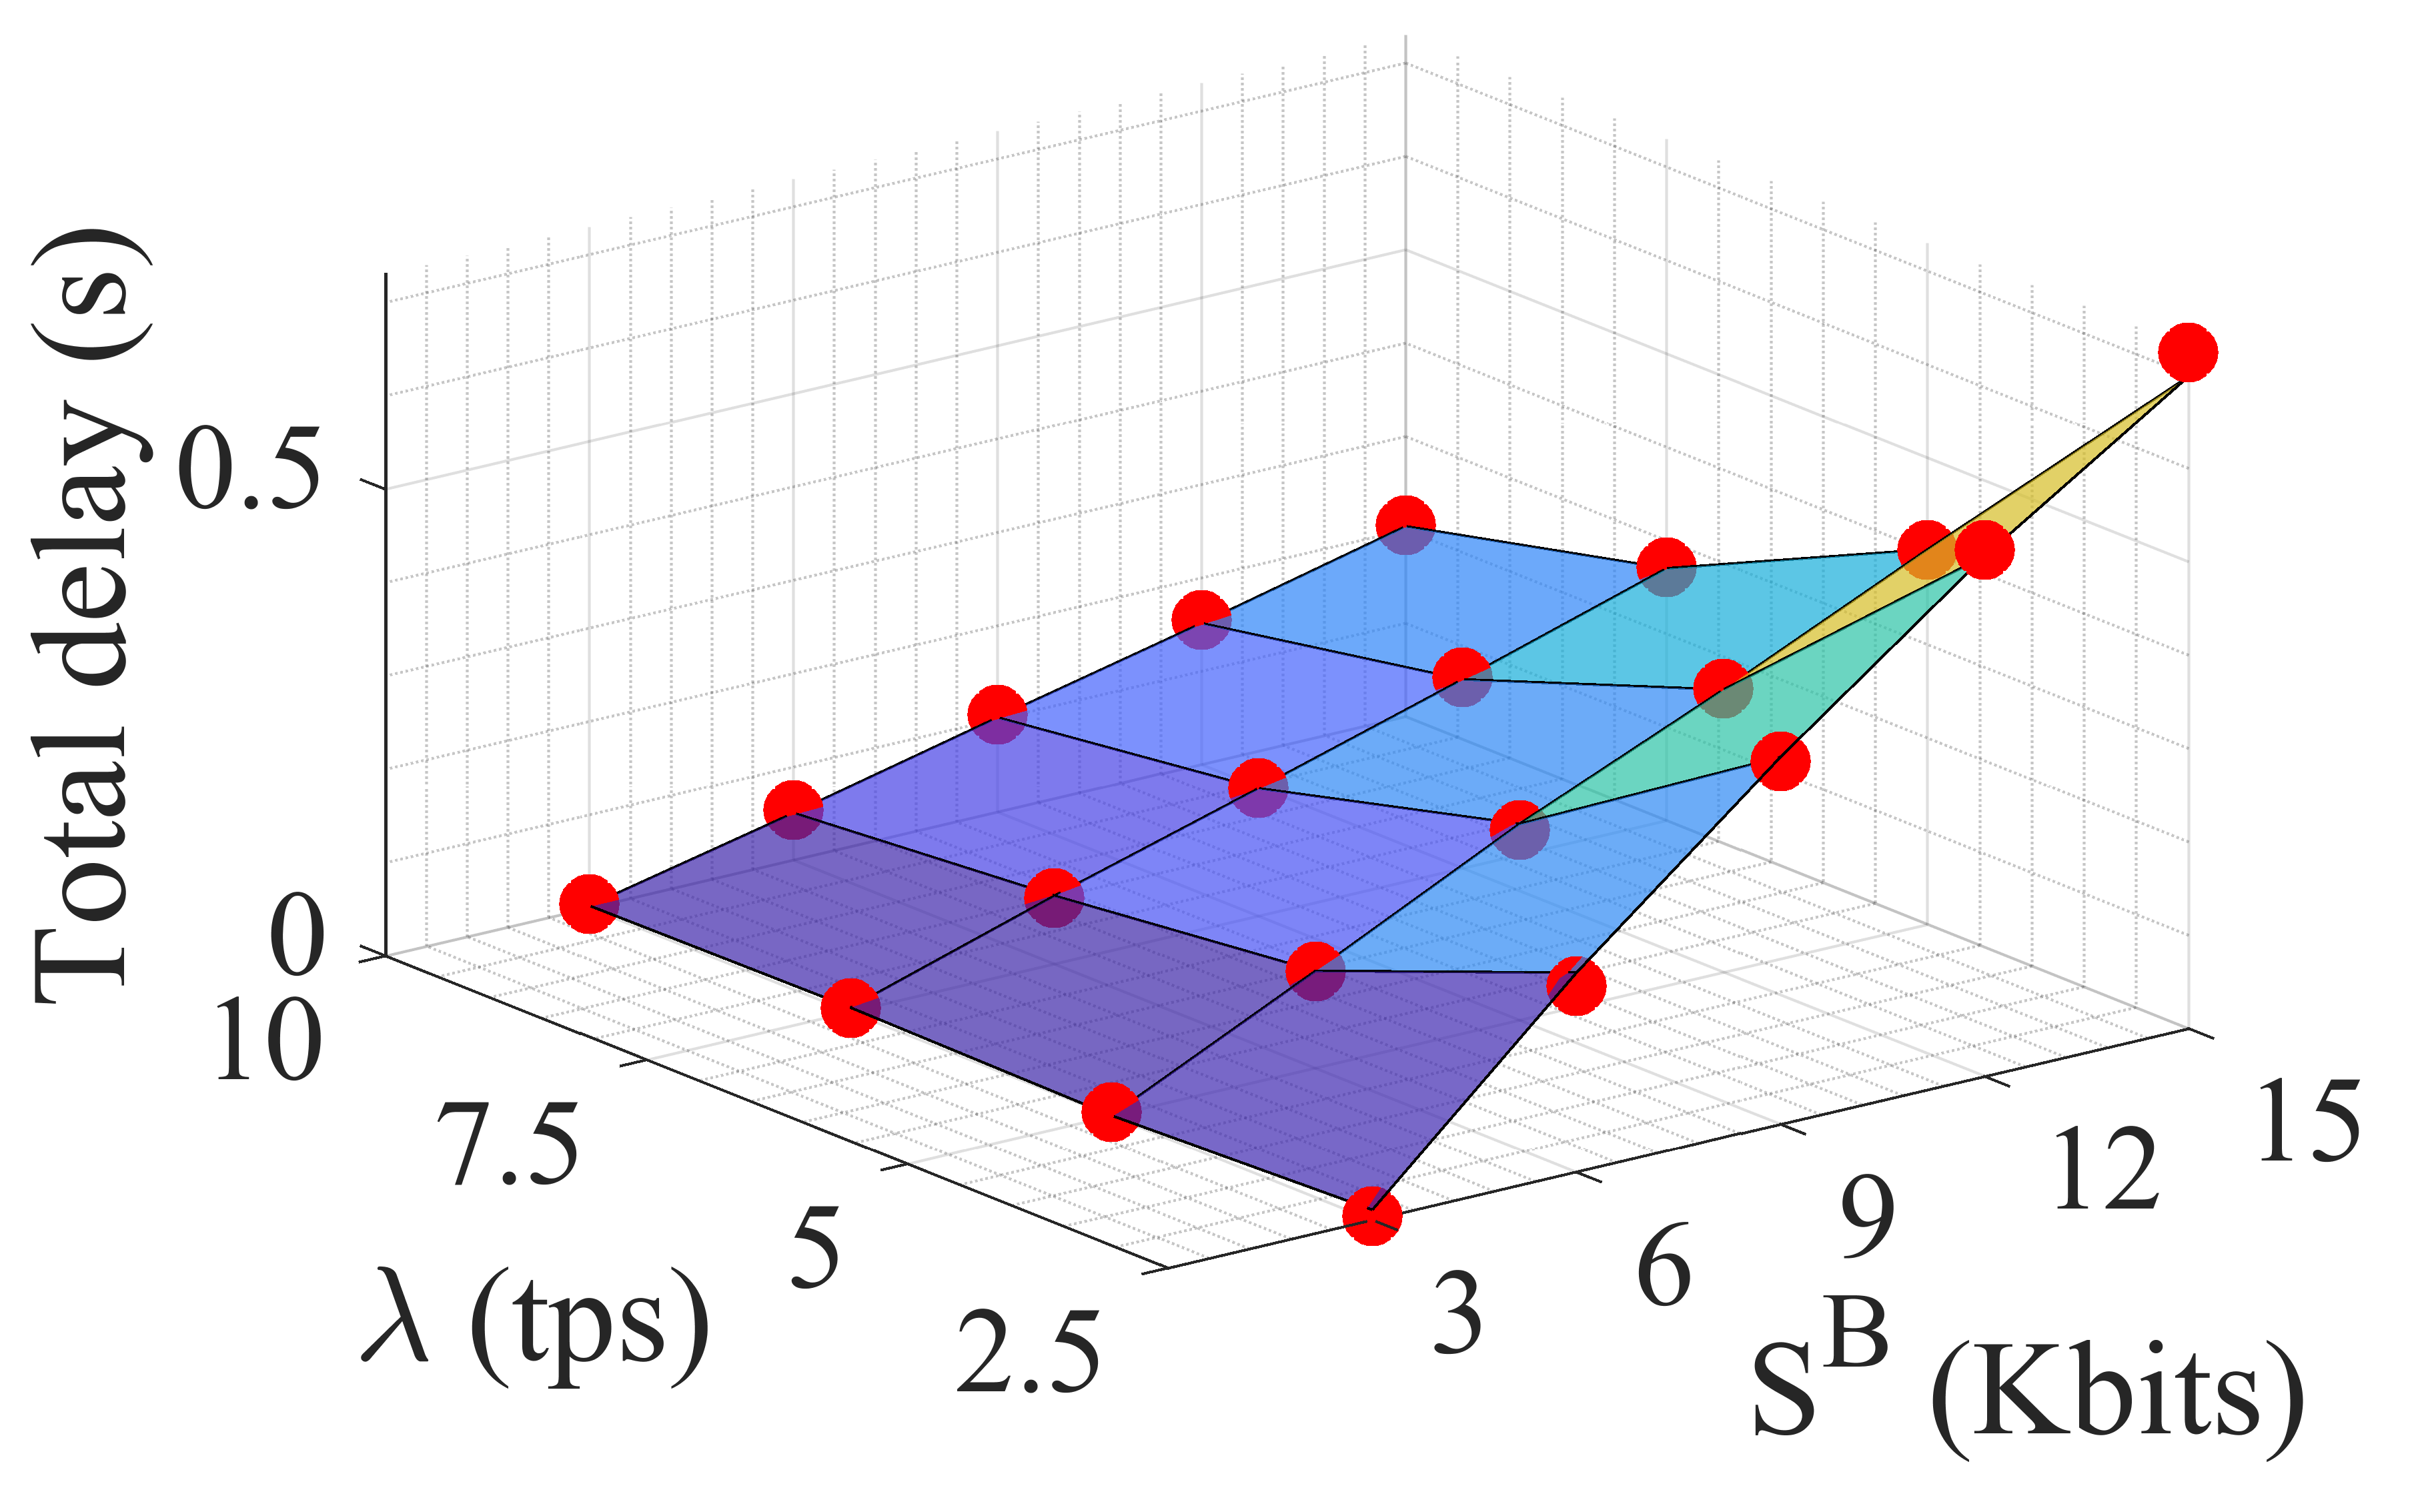
\includegraphics[width=0.7\textwidth,keepaspectratio]{img/total_delay_forks1_tw2}\caption{\scriptsize $T_w=2$ s, forks enabled}
		\end{figure}
	\end{column}
\end{columns}
\end{frame}

\subsection{}
\begin{frame}{Analysis of the queuing delay}
\begin{columns}
	\begin{column}{5.5cm}
		\begin{itemize}
			\item Impact of $\lambda$, $S^B$ and $T_w$
			\item Closed-form results
			\item Averaged results for $\lambda = \{2.5,5,7.5,10,12.5,15\}$
		\end{itemize}
	\end{column}
	\begin{column}{6cm}
		\begin{figure}
			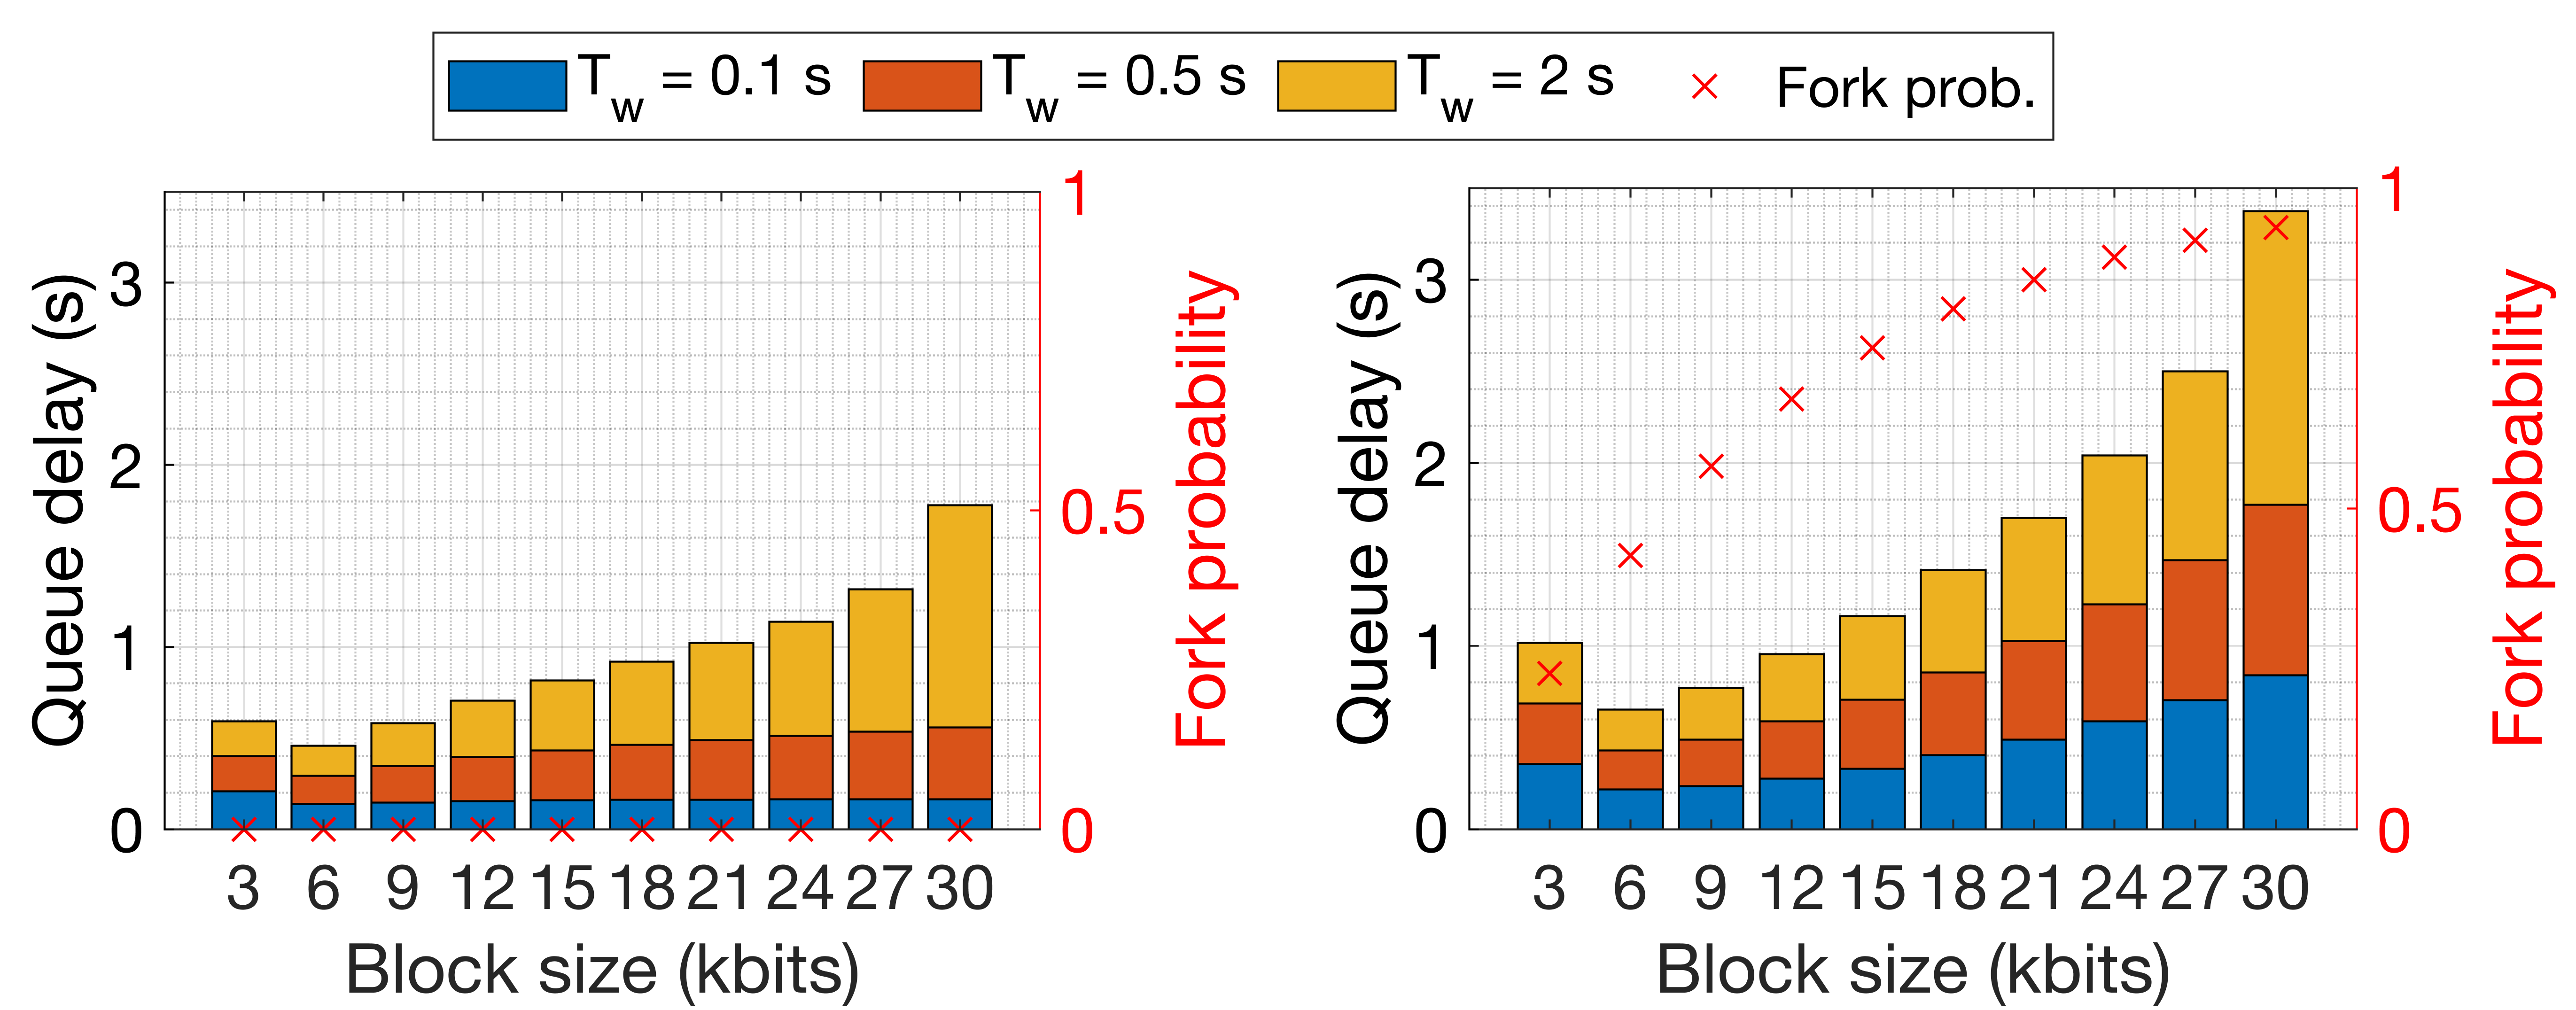
\includegraphics[width=1\textwidth,keepaspectratio]{img/queue_delay}\caption{\scriptsize Queuing delay}
		\end{figure}
		\vspace{-0.75cm}
		\begin{figure}
			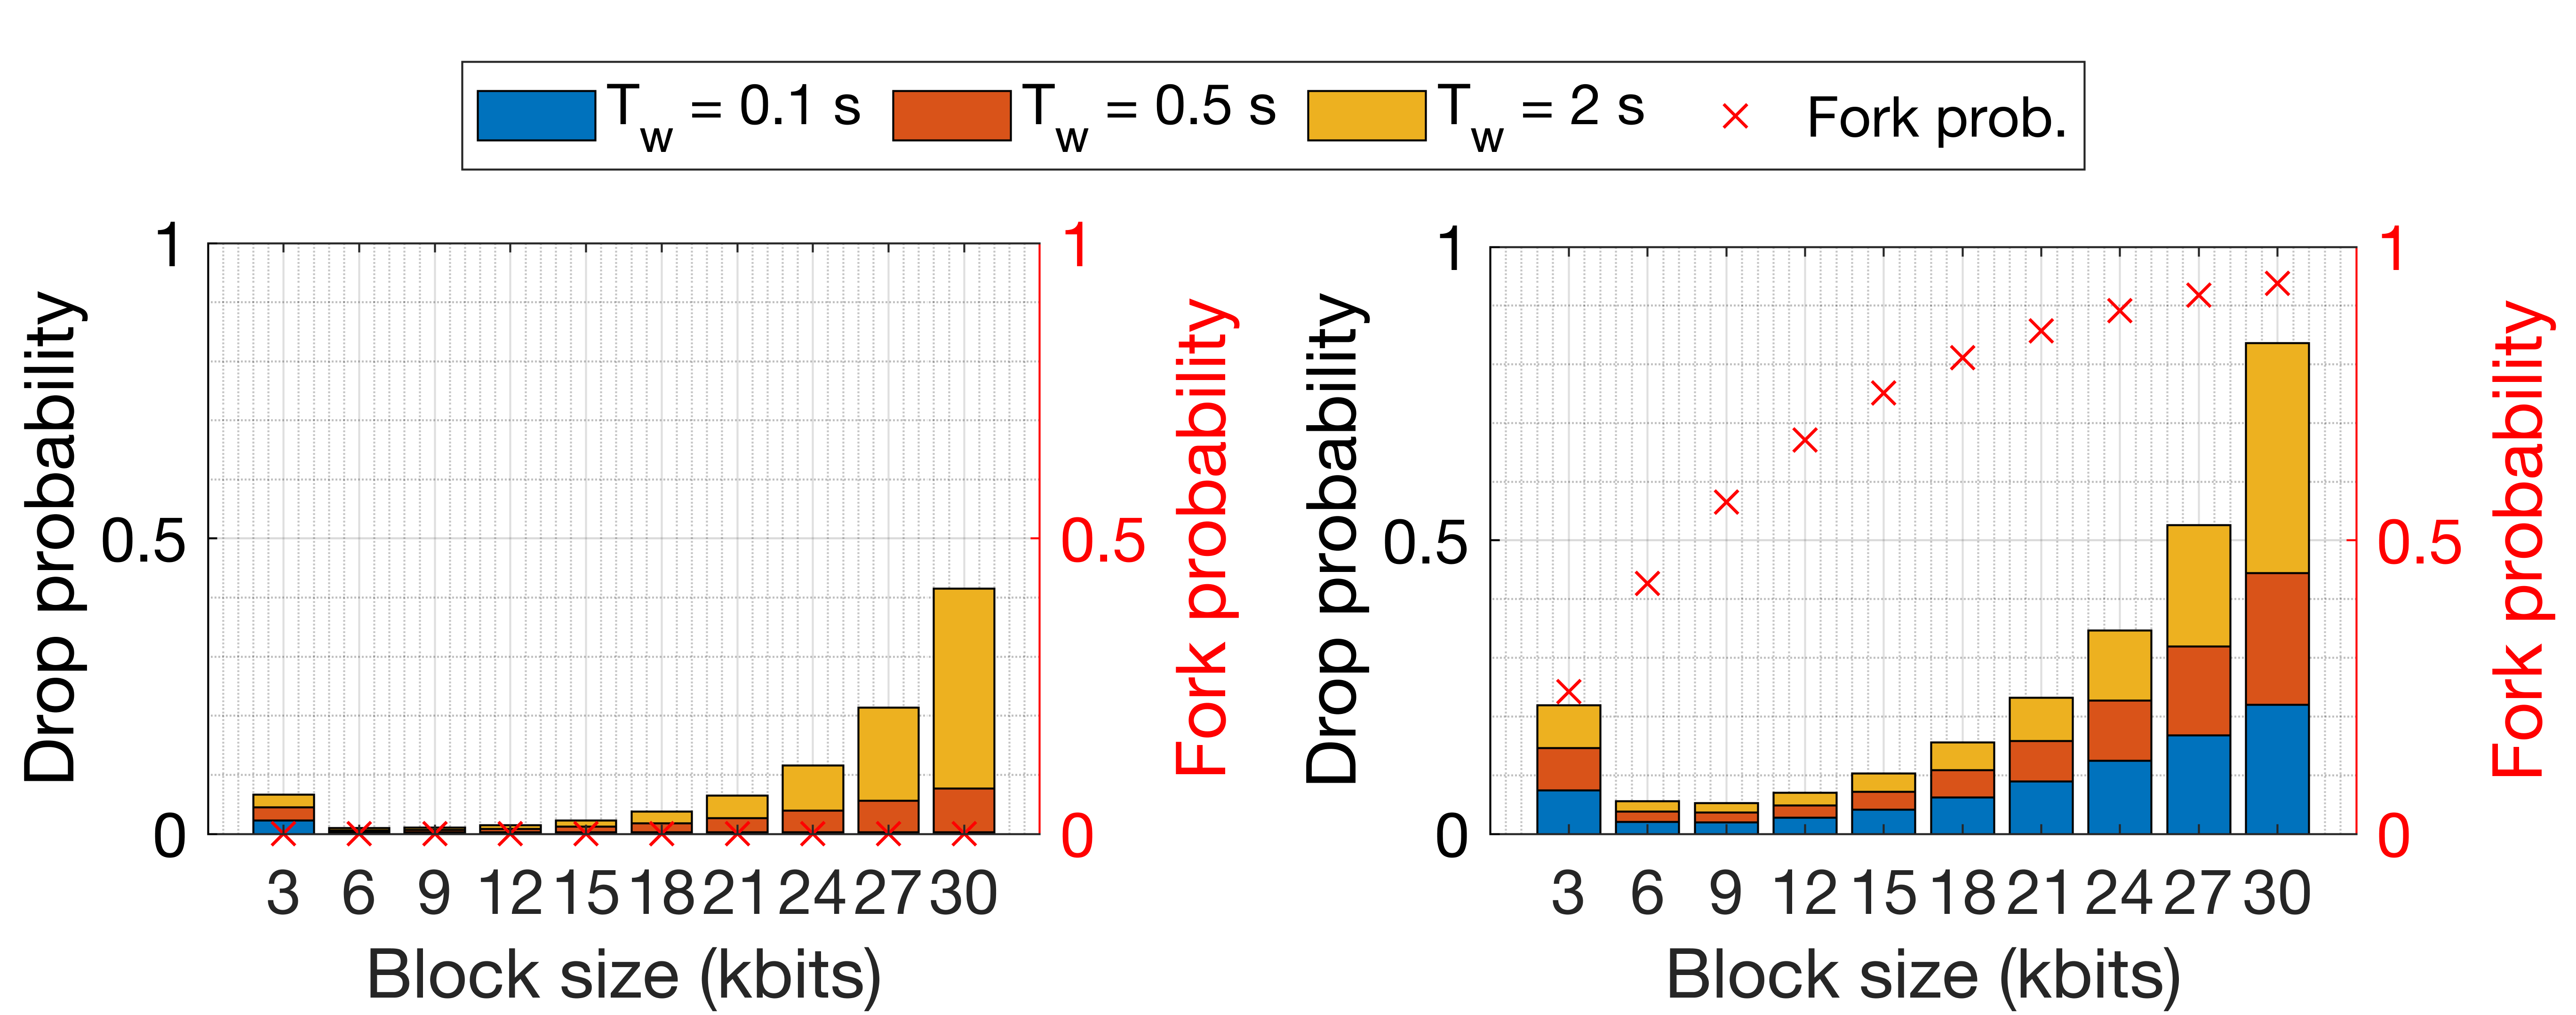
\includegraphics[width=1\textwidth,keepaspectratio]{img/drop_prob}\caption{\scriptsize Drop probability}
		\end{figure}
	\end{column}
\end{columns}
\end{frame}

\subsection{}
\begin{frame}{Transaction confirmation latency}
\begin{columns}
	\begin{column}{5.8cm}
		\begin{itemize}
			\item 5-30 concurrent STAs
			\item Full-buffer UDP-like traffic
			\item Block size ($S^B$) fixed to 6~Kbits
			\item Arrivals rate ($\lambda$) fixed to 7.5
			\item 10 random deployments
		\end{itemize}
	\end{column}
	\begin{column}{5.8cm}
		\begin{figure}
			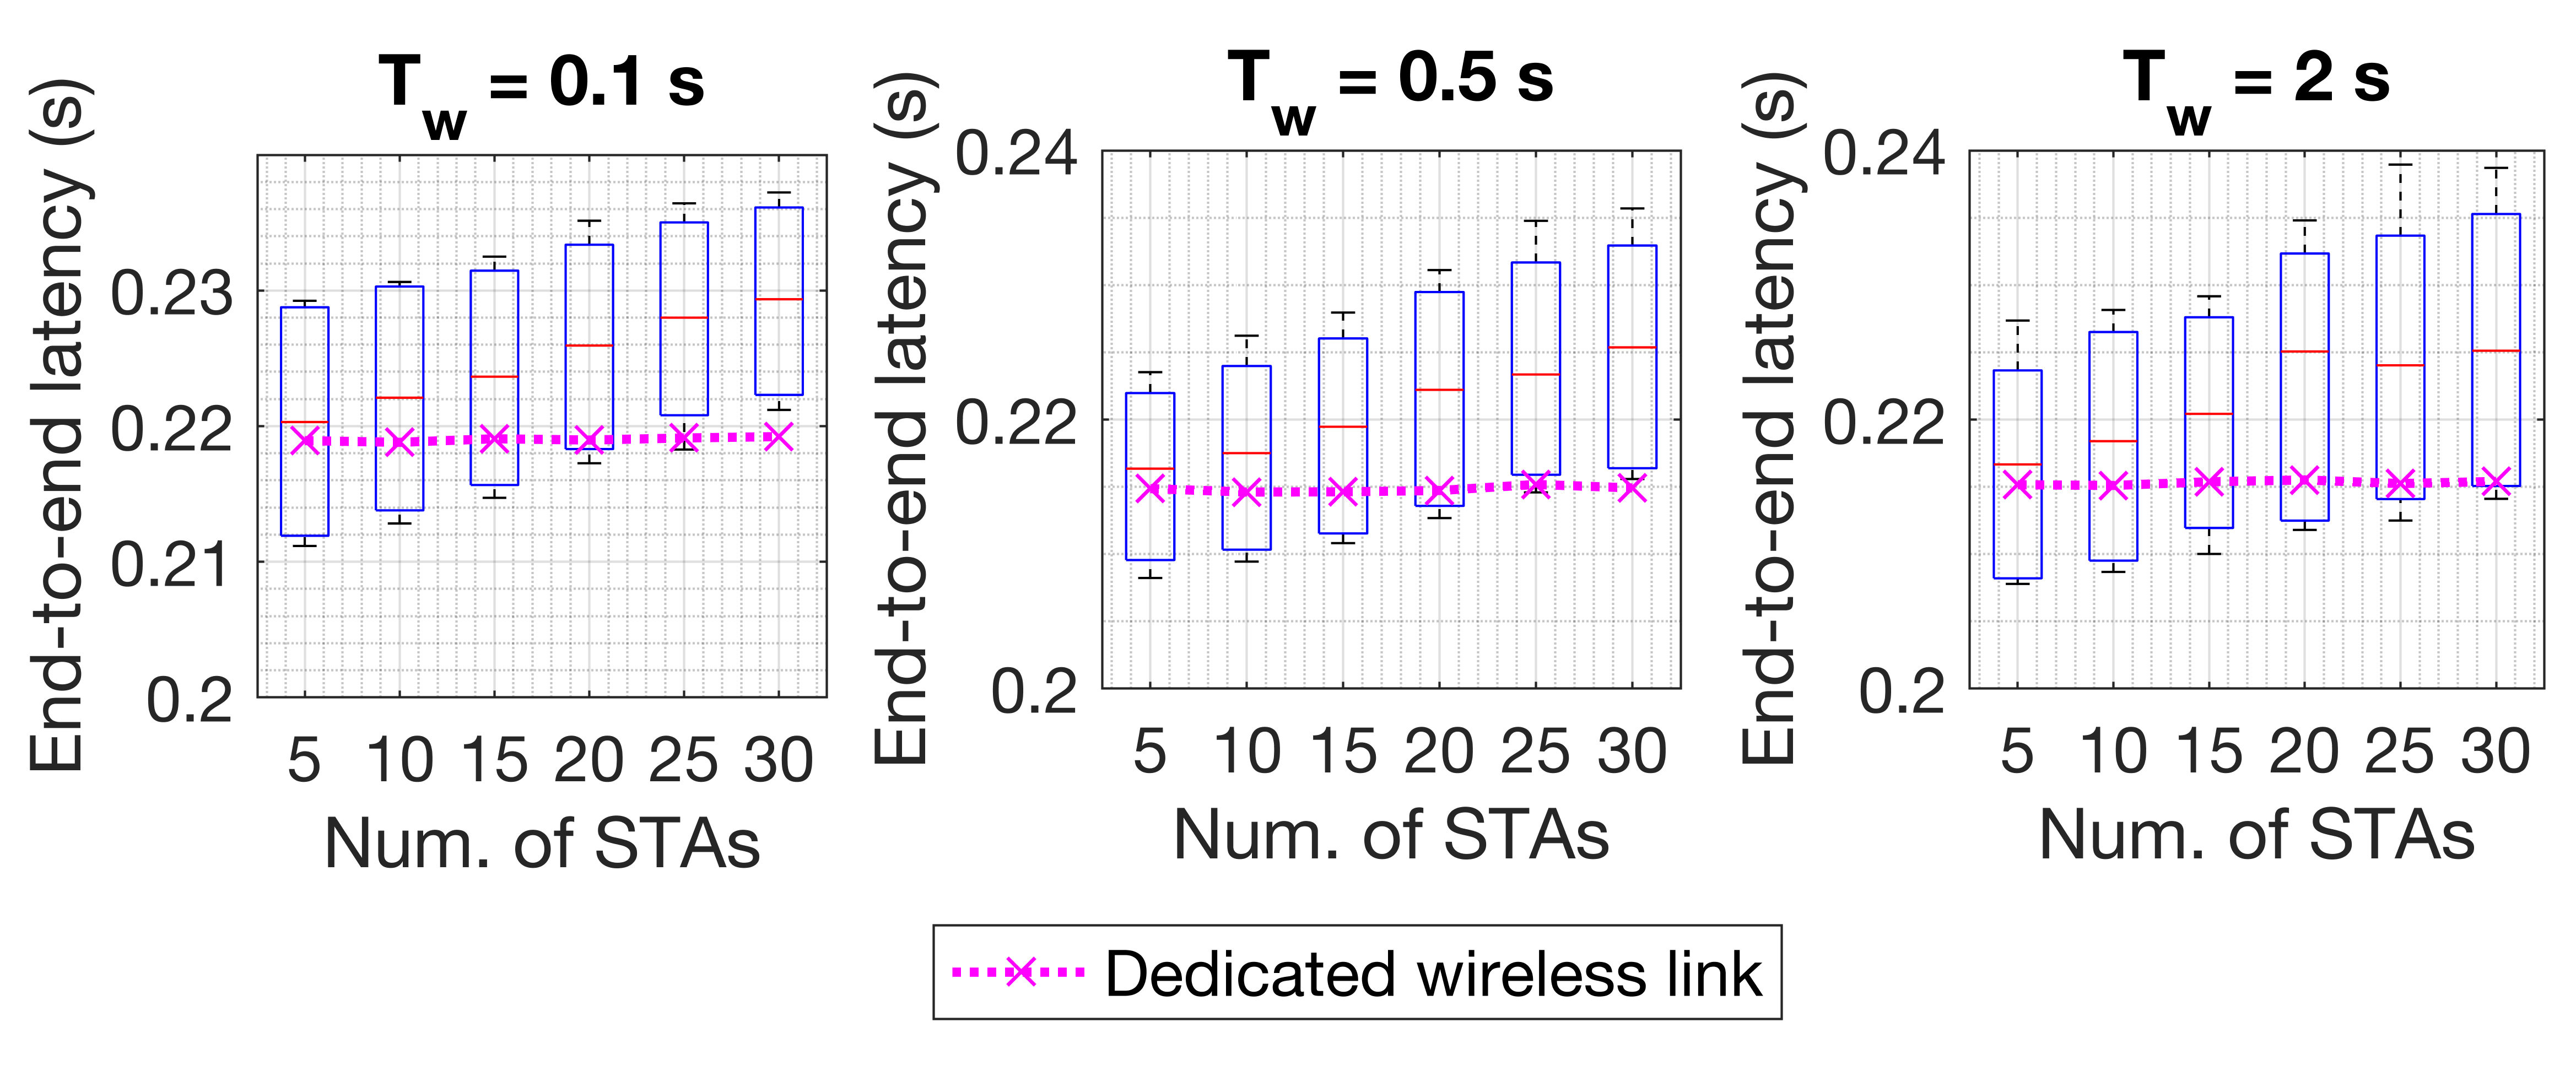
\includegraphics[width=1\textwidth,keepaspectratio]{img/delay_forks_disabled}\caption{Forks disabled}
		\end{figure}
		\vspace{-1cm}
		\begin{figure}
			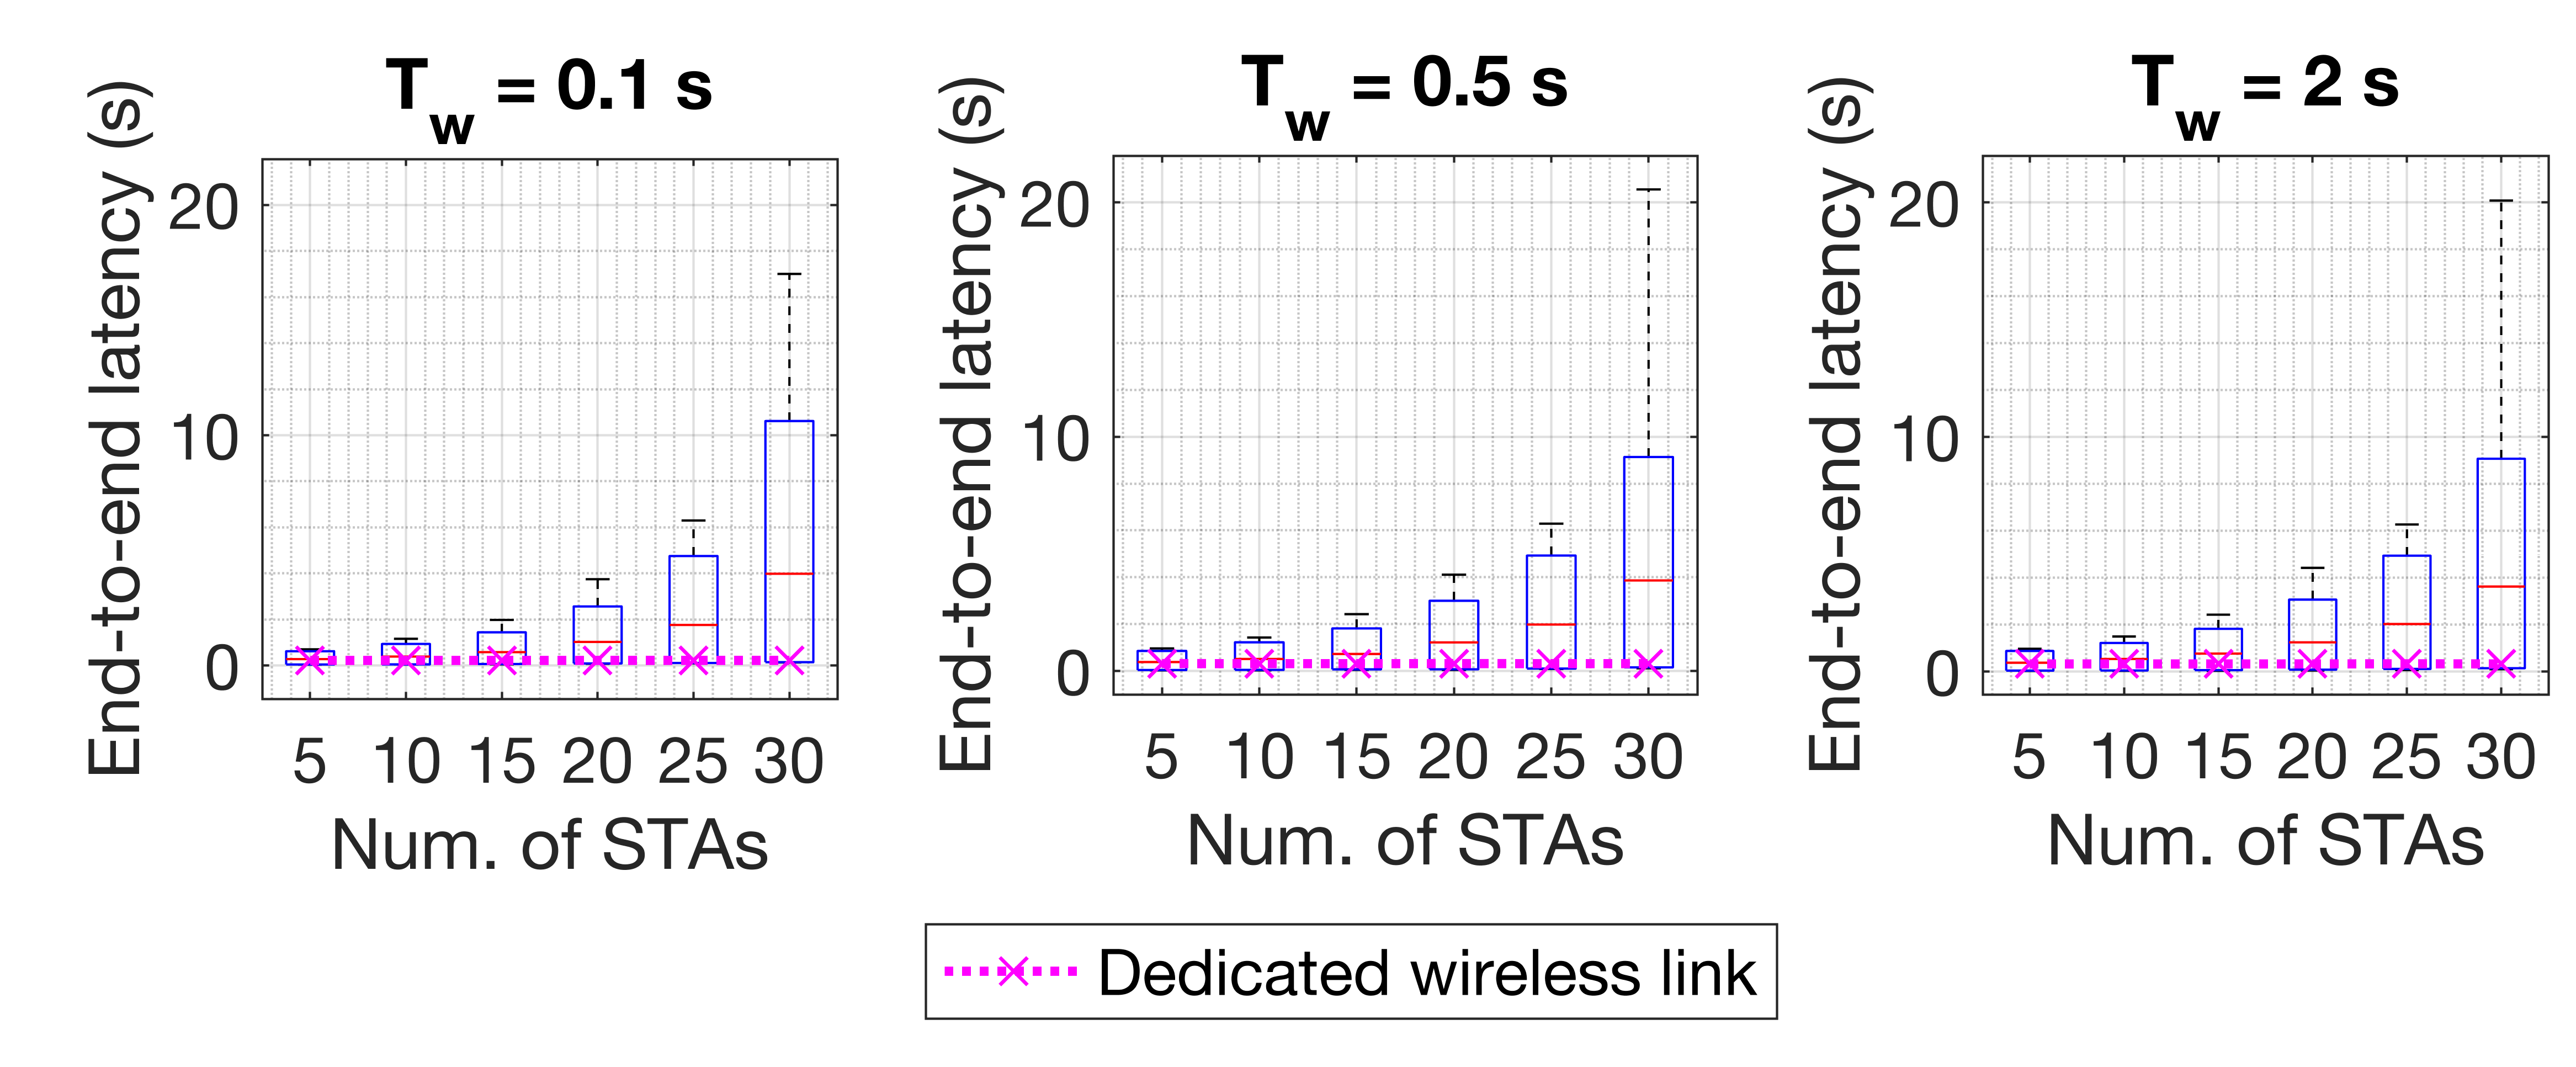
\includegraphics[width=1\textwidth,keepaspectratio]{img/delay_forks_enabled}\caption{Forks enabled}
		\end{figure}
	\end{column}
\end{columns}
\end{frame}

%%%%%%%%%%%%%%
%%% CONCLUSIONS
%%%%%%%%%%%%%%
\section{Conclusions}

\section{}
\begin{frame}{Some conclusions}
\begin{itemize}
	\item Future communications enabled by BC % where users are not bound to a specific operator and apply for resources through smart contracts	
	%BC allows secure and decentralized transactions among users and operators, but 
%	\item The BC latency represents a challenge %for the service perception of the UE and for the stability of the BC%, which will increasingly suffer from forks as the latency augments.
	\item Novel queue model for the BC delay, including timers and forks %our model perfectly captures the behaviors of the wireless BC
	\item Analysis on the performance of the wireless BC network
	\item Future work:
	\begin{itemize}
		\item Model packet losses
		\item Model re-transmissions
		\item Model burst arrivals
		\item Model different types of transactions %with different lengths
	\end{itemize}
\end{itemize}
\end{frame}

%%% Questions
\section{}
\begin{frame}{Questions}
\begin{figure}
	
\includegraphics[width=\textwidth,height=0.4\textheight,keepaspectratio]{img/question_mark.png}
\end{figure}

\begin{center}
	\footnotesize
	\textbf{Francesc Wilhelmi, Ph.D.}\\
	\textcolor{blue}{fwilhelmi@cttc.cat}\\
	Centre Tecnològic de Telecomunicacions de Catalunya (CTTC)\\
	%Universitat Pompeu Fabra (Barcelona)
\end{center}

\end{frame}

% References 
\begin{frame}[allowframebreaks]{References}
\scriptsize
\bibliographystyle{amsalpha}
\bibliography{bib}
\end{frame}

\end{document}